\documentclass[12pt,a4paper,openright,oneside]{book}
\usepackage[margin=1in]{geometry}

%------------------------------------------------
% Encoding and typography
%------------------------------------------------
\usepackage[T1]{fontenc}
\usepackage[utf8]{inputenc} % Remove if using LuaLaTeX/XeLaTeX
\usepackage{lmodern}
\usepackage{microtype}
\usepackage{setspace}
\onehalfspacing

%------------------------------------------------
% Graphics
%------------------------------------------------
\usepackage{graphicx}
\usepackage{pgfplots}
\usepackage{float}
\pgfplotsset{compat=1.18}

%------------------------------------------------
% Tables and layout
%------------------------------------------------
\usepackage{booktabs}
\usepackage{array}
\usepackage{longtable}
\usepackage{multicol}
\usepackage{changepage}
\usepackage{indentfirst}

%------------------------------------------------
% Code listings
%------------------------------------------------
\usepackage{listings}

%------------------------------------------------
% References
%------------------------------------------------
\usepackage{csquotes}
\usepackage[backend=biber, style=numeric]{biblatex}


%------------------------------------------------
% Hyperlinks
%------------------------------------------------
\usepackage[hidelinks]{hyperref}

%------------------------------------------------
% Document information
%------------------------------------------------
\title{Penetration Testing Report}
\author{Mariano Aponte}
\date{July 2026}

\usepackage[nottoc]{tocbibind}
% Definizione dei margini della pagina

\setlength{\parindent}{0pt}


\addbibresource{references.bib}

\begin{document}

%------------------------------------------------
% Front matter
%------------------------------------------------
\pagenumbering{gobble}
\begin{titlepage}
\centering

{\LARGE\textsc{University of Salerno}\par}
\vspace{0.2cm}

{\LARGE\textsc{Master's Degree in Computer Science}\par}
\vspace{0.2cm}

{\Large\textsc{Curriculum of Cybersecurity}\par}

\vspace{1cm}


\includegraphics[scale=0.35]{GlobalAssets/unisa_logo.png}

\vspace{1cm}



{\textsc{Project for the Penetration Testing and Ethical Hacking Exam}\par}

{\LARGE\textsc{Penetration Testing Report}\par}

\vspace{0.4cm}

{\LARGE\bfseries Corrosion: 1\par}

\vfill\vfill

\begin{minipage}{0.45\textwidth}
\raggedright
\textsc{Professor}\\
Arcangelo Castiglione
\end{minipage}
\hfill
\begin{minipage}{0.45\textwidth}
\raggedleft
\textsc{Student}\\
Mariano Aponte\\
Student ID: 0522501877
\end{minipage}

\vfill\vfill\vfill

{\large Academic Year 2025--2026\par}

\end{titlepage}

\clearpage

\tableofcontents

\clearpage
%------------------------------------------------
% Main matter
%------------------------------------------------
\pagenumbering{arabic}

\chapter{Executive Summary}

\section{Overview}
This report presents the results of the penetration testing engagement conducted by the student \textbf{Mariano Aponte}, with student ID \textbf{522501877} for the \textbf{Penetration Testing and Ethical Hacking exam}. 
\\

The assessment was carried out between \textbf{August 1, 2026} and \textbf{August 30, 2026}, and targeted the \textbf{"Corrosion: 1"} asset, a deliberately vulnerable system available on the VulnHub platform \cite{vulnhubCorrosion}.
\\

The objective of the assessment was to evaluate the security posture of the asset by identifying vulnerabilities that could be exploited by a malicious actor.
\\

The assessment was performed using a combination of automated and manual testing techniques, in a black-box fashion. The methodology was aligned with the \textbf{Penetration Testing Execution Standard (PTES)} \cite{ptes}. 
\\

All the testing activities were performed in accordance to the Rules of Engagement agreed by both parties, available in the Engagement Highlights section.
\\

The information available in this document is meant to be interpreted as educational only. All the penetration testing activities were carried out for educational purposes. No third parties assets were harmed or tested without explicit authorization.

\section{Overall Assessment}

The assessment identified \textbf{89 vulnerabilities} of the following severity:
\\


\begin{center}
	\begin{tabular}{lr}
		\toprule
		\textbf{Severity} & \textbf{Count} \\
		\midrule
		Critical & 21 \\
		High & 45 \\
		Medium & 19 \\
		Low & 0 \\
		Not Rated/Info & 4 \\
		\bottomrule
	\end{tabular}
\end{center}

Several of these vulnerabilities were successfully chained during exploitation, ultimately resulting in complete compromise of the target system.
\\

Based on the number and severity of identified vulnerabilities and the successful compromise of the host, the overall security posture is assessed as \textbf{Unacceptable}.

\section{Key Findings}

The most significant findings identified during the assessment include:

\begin{enumerate}
\item \textbf{Critical: Web Application Vulnerability Leading to Remote Access}

A vulnerability in the web application allows unauthorized access to sensitive files and can be subsequently used to execute commands on the server. This weakness could provide an attacker with \textbf{remote access to the system}.

\item \textbf{Critical: Outdated Apache HTTP Server with Known Vulnerabilities}

The target runs \texttt{Apache HTTP Server 2.4.46}, an outdated version affected by multiple known vulnerabilities. Depending on the enabled modules and configuration, these vulnerabilities could lead to denial of service and/or remote code execution.

\item \textbf{Critical: Local Privilege Escalation}

A user utility has excessive privileges and could be manipulated to execute unauthorized commands with \textbf{root-level privileges}. This weakness could allow an attacker to escalate from a standard user account to full administrative access.

\item \textbf{High: Exposure of Sensitive Files and Authentication Information}

Several files are accessible through the web application and can disclose information useful for further attacks. In particular, the application exposes \texttt{/var/log/auth.log}, which contains authentication activity, access attempts, and other security-relevant information.

\item \textbf{High: Weak Protection of Sensitive Backup Data and Credentials}

A password-protected backup archive containing user credentials is discovered on the system. The archive password is weak and can be easily cracked, allowing access to the stored credentials and subsequent authentication as the \texttt{randy} user.

\item \textbf{High: Vulnerable Linux Kernel / Missing Security Patches}

Manual analysis identified a Linux Kernel vulnerability that could allow a local user to gain higher privileges.
\end{enumerate}

Complete technical details and remediation recommendations are provided in the Vulnerability Report section.

\section{Recommendations}

To improve the overall security posture, the following actions are recommended:

\begin{enumerate}
    \item Apply vendor security updates and patches and keep the Operating System and the Apache2 Web Server up to date.
    \item Implement Secure Programming best practices for web-exposed and system applications.
    \item Strengthen password policy for both user accounts and protected files.
    \item Review privilege assignments for critical and high-risk executables and files.
    \item Enhance logging, monitoring, and incident detection capabilities.
    \item Perform regular vulnerability assessments and periodic penetration tests.
\end{enumerate}

\section{Conclusion}
\textbf{This report reflects the security posture of the assessed systems at the time of testing. Changes made to the environment after the assessment may affect the validity of these results. Continuous security monitoring and periodic reassessment are therefore always recommended.}
\clearpage

\chapter{Engagement Highlights} \label{highlights}
\section{Overview}
This chapter defines the Rules of Engagement (RoE) for the penetration testing activity performed as part of the Penetration Testing and Ethical Hacking exam.

\section{Purpose and Objectives}
The purpose of this penetration testing activity is to evaluate the security posture of the intentionally vulnerable virtual machine \textbf{"Corrosion: 1"}.
\\

The penetration testing activities is performed in a black-box fashion.
\\

The activity is conducted as part of the Penetration Testing and Ethical Hacking exam and aims to demonstrate practical knowledge of offensive security methodologies.
\\

The objectives of the assessment are:

\begin{itemize}
    \item Identify security vulnerabilities present within the target system.
    \item Perform reconnaissance and enumeration activities.
    \item Exploit discovered vulnerabilities where technically feasible.
    \item Demonstrate penetration testing methodologies and techniques.
    \item Document discovered vulnerabilities, exploitation procedures,
    evidence, and remediation recommendations.
\end{itemize}

The penetration test is conducted exclusively for educational purposes within an authorized laboratory environment.

\section{Scope of Testing}
\subsection{In-Scope Assets}
The following asset is explicitly authorized for testing:

\begin{itemize}
    \item \textbf{Target:} Corrosion: 1 virtual machine.
    \item \textbf{Environment:} Isolated virtual laboratory network.
\end{itemize}

All services, applications, configurations, user accounts, and files contained inside the target virtual machine are considered within scope.

\subsection{Out-of-Scope Assets}
The following assets are explicitly excluded from the scope:

\begin{itemize}
    \item The physical host machine running the virtualization software.
    \item Other virtual machines present in the laboratory environment.
    \item External networks and Internet-accessible systems.
    \item Any system not explicitly identified as the target machine.
\end{itemize}

No testing activity shall intentionally affect systems outside the authorized
scope.


\section{Authorized Testing Activities}
The following activities are authorized against the target virtual machine:

\begin{itemize}
    \item Network discovery and host identification.
    \item Port scanning and service enumeration.
    \item Vulnerability identification and assessment.
    \item Web application testing.
    \item Configuration analysis.
    \item Credential testing against exposed services.
    \item Controlled exploitation of identified vulnerabilities.
    \item Privilege escalation attempts.
    \item Post-exploitation analysis limited exclusively to the target machine.
    \item Collection of technical evidence for reporting purposes.
\end{itemize}

Since the target machine is intentionally vulnerable and isolated, exploitation activities are permitted when required to demonstrate penetration testing techniques.

\section{Prohibited Activities}
The following actions are prohibited:

\begin{itemize}
    \item Attacking systems outside the defined scope.
    \item Performing denial-of-service attacks against external systems.
    \item Modifying or damaging the host operating system.
    \item Performing security tests against third-party infrastructure.
\end{itemize}

\section{Testing Methodology}
\subsection{Methodology}
The penetration testing activities will be conducted in accordance with the \textit{Penetration Testing Execution Standard (PTES)}. 
\\

PTES provides a structured framework for planning, executing, and documenting penetration tests, ensuring that the assessment follows a consistent and methodical approach. 
\\

The methodology encompasses the relevant phases of the penetration testing process, including pre-engagement interactions, intelligence gathering, threat modelling, vulnerability analysis, exploitation, post-exploitation, and reporting \cite{ptes}. 

\subsection{Tools}
The following tools were used during the assessment:

\begin{itemize}
	\item Oracle VirtualBox \cite{virtualbox};
	\item Kali Linux \cite{kali};
    \item \texttt{nmap} \cite{nmap};
    \item \texttt{DirBuster} \cite{dirbuster};
    \item \texttt{Gobuster} \cite{gobuster};
    \item \texttt{wfuzz} \cite{wfuzz};
    \item \texttt{Nessus} \cite{nessus};
    \item \texttt{Nikto} \cite{nikto};
    \item \texttt{WafW00f} \cite{wafwoof};
    \item \texttt{Exploit Database} \cite{exploitdb};
    \item \texttt{Metasploit} \cite{metasploitMetasploitPenetration};
    \item \texttt{ssh} and \texttt{sftp} \cite{ssh};
    \item \texttt{curl} \cite{curl};
    \item \texttt{zip2john} and \texttt{john} \cite{john};
    \item \texttt{C} \cite{c}, \texttt{PHP} \cite{php} and \texttt{Python} \cite{python} programming;
    \item \texttt{netcat} \cite{netcat};
    \item \texttt{WeBaCoo} \cite{webacoo}.
\end{itemize}

\section{Data Handling}
Information collected during the penetration test shall be handled responsibly.
\\

The tester agrees to:

\begin{itemize}
    \item Use collected information only for academic evaluation purposes.
    \item Preserve only evidence required for the final report.
    \item Remove temporary testing artifacts when possible.
\end{itemize}

\section{Risk Management}
Although the target system is intentionally vulnerable, penetration testing
activities may cause service interruption, system instability, or modification
of data contained within the virtual machine.
\\

The tester is responsible for maintaining the isolation of the laboratory
environment and ensuring that testing activities remain limited to the
authorized target.
\\

Virtual machine snapshots may be used to restore the environment if necessary.

\section{Reporting and Communication}
The final penetration testing report will contain:

\begin{itemize}
    \item Scope and methodology.
    \item Tools and techniques used.
    \item Identified vulnerabilities.
    \item Exploitation procedures.
    \item Evidence of successful exploitation.
    \item Security impact analysis.
    \item Recommended mitigation strategies.
\end{itemize}

The report will be submitted to Prof. Arcangelo Castiglione as part of the
Penetration Testing and Ethical Hacking examination.

\section{Duration of Testing}

Testing activities are authorized during the exam period assigned by the
course supervisor.
\\

The tester may perform penetration testing activities against the target
virtual machine during this period, provided that all rules defined in this
document are followed.

\section{Authorization}
This section provides formal authorization for the tester to perform
penetration testing activities against the specified target system, within the scope and limitations described in this chapter.
\clearpage

\chapter{Vulnerability Report}

\section{Overview}

This chapter provides a high-level summary of the vulnerabilities identified during the penetration test, including their severity and CVE references. 

\section{Key Findings}

The assessment identified \textbf{89 vulnerabilities}; the most significant findings include:

\begin{enumerate}
	\item \textbf{Critical: Web Application Vulnerability Leading to Remote Access}
	
	A vulnerability in the web application allows unauthorized access to sensitive files and can be subsequently used to execute commands on the server. This weakness could provide an attacker with \textbf{remote access to the system}.
	
	\item \textbf{Critical: Outdated Apache HTTP Server with Known Vulnerabilities}
	
	The target runs \texttt{Apache HTTP Server 2.4.46}, an outdated version affected by multiple known vulnerabilities. Depending on the enabled modules and configuration, these vulnerabilities could lead to denial of service and/or remote code execution.
	
	\item \textbf{Critical: Local Privilege Escalation}
	
	A user utility has excessive privileges and could be manipulated to execute unauthorized commands with \textbf{root-level privileges}. This weakness could allow an attacker to escalate from a standard user account to full administrative access.
	
	\item \textbf{High: Exposure of Sensitive Files and Authentication Information}
	
	Several files are accessible through the web application and can disclose information useful for further attacks. In particular, the application exposes \texttt{/var/log/auth.log}, which contains authentication activity, access attempts, and other security-relevant information.
	
	\item \textbf{High: Weak Protection of Sensitive Backup Data and Credentials}
	
	A password-protected backup archive containing user credentials is discovered on the system. The archive password is weak and can be easily cracked, allowing access to the stored credentials and subsequent authentication as the \texttt{randy} user.
	
	\item \textbf{High: Vulnerable Linux Kernel / Missing Security Patches}
	
	Manual analysis identified a Linux Kernel vulnerability that could allow a local user to gain higher privileges through mishandling of user namespace mapping.
\end{enumerate}

\section{Vulnerability Index}

\begin{longtable}{|l|p{5cm}|l|l|p{3cm}|}
\hline
\textbf{ID} & \textbf{Finding} & \textbf{Severity} & \textbf{CVE} & \textbf{Affected Asset} \\ \hline
F-001 & Sensitive Information Exposure in Public Web Root & 8.6 HIGH & N/A & Web App exposed by Apache2 HTTP Web Server \\ \hline
F-002 & Local File Inclusion (LFI) via Path Traversal & 8.6 HIGH & N/A & randylogs.php \\ \hline
F-003 & Log Poisoning via Unsanitized SFTP Authentication Input & 9.3 CRITICAL & N/A & SFTP and /var/log/auth.log \\ \hline
F-004 & Insecure Local Permissions on Backup Artifacts & 5.3 MEDIUM & N/A & user\_backup.zip file \\ \hline
F-005 & Weak Password Architecture on Backup Archives & 7.8 HIGH & N/A & user\_backup.zip file \\ \hline
F-006 & Local Privilege Escalation via SUID Binary Search Path Hijacking & 8.8 HIGH & N/A & easysysinfo executable \\ \hline
F-007 & HTTP Request Splitting / Smuggling with mod\_rewrite and mod\_proxy & 9.8 CRITICAL & CVE-2023-25690 & Apache2 HTTP Web Server \\ \hline
F-008 & mod\_proxy\_uwsgi HTTP Response Splitting & 7.5 HIGH & CVE-2023-27522 & Apache2 HTTP Web Server \\ \hline
F-009 & WebSocket Protocol Upgrade Null Pointer Dereference & 5.4 MEDIUM & CVE-2024-36387 & Apache2 HTTP Web Server \\ \hline
F-010 & SSRF in Apache HTTP Server on Windows NTLM Hash Leakage & 7.5 HIGH & CVE-2024-38472 & Apache2 HTTP Web Server\\ \hline
F-011 & mod\_proxy Request URL Encoding Authentication Bypass & 8.1 HIGH & CVE-2024-38473 & Apache2 HTTP Web Server\\ \hline
F-012 & mod\_rewrite Substitution Encoding Script Execution / Source Disclosure & 9.8 CRITICAL & CVE-2024-38474 & Apache2 HTTP Web Server\\ \hline
F-013 & mod\_rewrite Output Escaping File Mapping Vulnerability & 9.1 CRITICAL & CVE-2024-38475 & Apache2 HTTP Web Server\\ \hline
F-014 & Core Information Disclosure / SSRF / Script Execution & 9.8 CRITICAL & CVE-2024-38476 & Apache2 HTTP Web Server\\ \hline
F-015 & mod\_proxy Null Pointer Dereference Denial of Service & 7.5 HIGH & CVE-2024-38477 & Apache2 HTTP Web Server\\ \hline
F-016 & mod\_rewrite Potential SSRF via mod\_proxy & 7.5 HIGH & CVE-2024-39573 & Apache2 HTTP Web Server\\ \hline
F-017 & HTTP/2 Protocol Double Free and Remote Code Execution & 8.8 HIGH & CVE-2026-23918 & Apache2 HTTP Web Server\\ \hline
F-018 & Local .htaccess Authors Escalation of Privilege & 8.8 HIGH & CVE-2026-24072 & Apache2 HTTP Web Server\\ \hline
F-019 & mod\_proxy\_ajp Heap-based Buffer Overflow & 9.8 CRITICAL & CVE-2026-28780 & Apache2 HTTP Web Server\\ \hline
F-020 & mod\_md Resource Allocation Without Limits via OCSP & 7.3 HIGH & CVE-2026-29168 & Apache2 HTTP Web Server\\ \hline
F-021 & mod\_dav\_lock NULL Pointer Dereference & 7.5 HIGH & CVE-2026-29169 & Apache2 HTTP Web Server\\ \hline
F-022 & Apache 2.4.x $<$ 2.4.67 Vulnerability (CVE-2026-33006) & 4.8 MEDIUM & CVE-2026-33006 & Apache2 HTTP Web Server\\ \hline
F-023 & Apache 2.4.x $<$ 2.4.67 Vulnerability (CVE-2026-33007) & 5.3 MEDIUM & CVE-2026-33007 & Apache2 HTTP Web Server\\ \hline
F-024 & Apache 2.4.x $<$ 2.4.67 Vulnerability (CVE-2026-33523) & 6.5 MEDIUM & CVE-2026-33523 & Apache2 HTTP Web Server\\ \hline
F-025 & Apache 2.4.x $<$ 2.4.67 Vulnerability (CVE-2026-33857) & 5.3 MEDIUM & CVE-2026-33857 & Apache2 HTTP Web Server\\ \hline
F-026 & Apache 2.4.x $<$ 2.4.67 Vulnerability (CVE-2026-34032) & 5.3 MEDIUM & CVE-2026-34032 & Apache2 HTTP Web Server\\ \hline
F-027 & Apache 2.4.x $<$ 2.4.67 Vulnerability (CVE-2026-34059) & 7.5 HIGH & CVE-2026-34059 & Apache2 HTTP Web Server\\ \hline
F-028 & mod\_proxy\_wstunnel and mod\_proxy\_http Upgradable Protocols Negotiation & 5.3 MEDIUM & CVE-2019-17567 & Apache2 HTTP Web Server \\ \hline
F-029 & Windows Local Process Stopping Vulnerability & 5.5 MEDIUM & CVE-2020-13938 & Apache2 HTTP Web Server\\ \hline
F-030 & mod\_proxy\_http NULL Pointer Dereference Denial of Service & 7.5 HIGH & CVE-2020-13950 & Apache2 HTTP Web Server\\ \hline
F-031 & mod\_auth\_digest Stack Overflow via Digest Nonce & 7.3 HIGH & CVE-2020-35452 & Apache2 HTTP Web Server\\ \hline
F-032 & mod\_session NULL Pointer Dereference Denial of Service & 7.5 HIGH & CVE-2021-26690 & Apache2 HTTP Web Server\\ \hline
F-033 & mod\_session NULL Pointer Dereference DoS via SessionHeader & 9.8 CRITICAL & CVE-2021-26691 & Apache2 HTTP Web Server\\ \hline
F-034 & Unexpected $<$Location$>$ Section Matching with 'MergeSlashes OFF' & 5.3 MEDIUM & CVE-2021-30641 & Apache2 HTTP Web Server\\ \hline
F-035 & Apache 2.4.x $<$ 2.4.52 mod\_lua Buffer Overflow & 9.8 CRITICAL & CVE-2021-44790 & Apache2 HTTP Web Server\\ \hline
F-036 & mod\_lua Use of Uninitialized Value in r:parsebody & 7.5 HIGH & CVE-2022-22719 & Apache2 HTTP Web Server\\ \hline
F-037 & HTTP Request Smuggling Connection Closing Issue & 9.8 CRITICAL & CVE-2022-22720 & Apache2 HTTP Web Server\\ \hline
F-038 & LimitXMLRequestBody Integer Overflow / Out-of-bounds Write & 9.1 CRITICAL & CVE-2022-22721 & Apache2 HTTP Web Server\\ \hline
F-039 & mod\_sed Read/Write Beyond Bounds Heap Overwrite & 9.8 CRITICAL & CVE-2022-23943 & Apache2 HTTP Web Server\\ \hline
F-040 & Apache 2.4.x $<$ 2.4.54 Authentication Bypass via mod\_proxy & 9.8 CRITICAL & CVE-2022-31813 & Apache2 HTTP Web Server\\ \hline
F-041 & If: Request Header Heap Memory Read/Write & 7.5 HIGH & CVE-2006-20001 & Apache2 HTTP Web Server\\ \hline
F-042 & mod\_proxy\_ajp HTTP Request Smuggling & 9.0 CRITICAL & CVE-2022-36760 & Apache2 HTTP Web Server\\ \hline
F-043 & Backend Response Header Early Truncation & 5.3 MEDIUM & CVE-2022-37436 & Apache2 HTTP Web Server\\ \hline
F-044 & HTTP/2 Connection Block DoS via Initial Window Size 0 & 7.5 HIGH & CVE-2023-43622 & Apache2 HTTP Web Server\\ \hline
F-045 & HTTP/2 Stream Deferred Memory Release DoS & 5.9 MEDIUM & CVE-2023-45802 & Apache2 HTTP Web Server\\ \hline
F-046 & Apache 2.4.x $<$ 2.4.58 Out-of-Bounds Read (CVE-2023-31122) & 7.5 HIGH & CVE-2023-31122 & Apache2 HTTP Web Server\\ \hline
F-047 & HTTP Response Splitting in Multiple Modules & 7.3 HIGH & CVE-2023-38709 & Apache2 HTTP Web Server\\ \hline
F-048 & HTTP Response Splitting Desynchronization Attack & 6.3 MEDIUM & CVE-2024-24795 & Apache2 HTTP Web Server\\ \hline
F-049 & HTTP/2 DoS by Memory Exhaustion on Continuation Frames & 7.5 HIGH & CVE-2024-27316 & Apache2 HTTP Web Server\\ \hline
F-050 & Apache 2.4.x $<$ 2.4.68 Vulnerability (CVE-2026-29167) & 9.8 CRITICAL & CVE-2026-29167 & Apache2 HTTP Web Server \\ \hline
F-051 & Apache 2.4.x $<$ 2.4.68 Vulnerability (CVE-2026-29170) & 6.1 MEDIUM & CVE-2026-29170& Apache2 HTTP Web Server \\ \hline
F-052 & Apache 2.4.x $<$ 2.4.68 Vulnerability (CVE-2026-34355) & 7.5 HIGH & CVE-2026-34355 & Apache2 HTTP Web Server\\ \hline
F-053 & Apache 2.4.x $<$ 2.4.68 Vulnerability (CVE-2026-34356) & 7.5 HIGH & CVE-2026-34356 & Apache2 HTTP Web Server\\ \hline
F-054 & Apache 2.4.x $<$ 2.4.68 Vulnerability (CVE-2026-42535) & 9.1 CRITICAL & CVE-2026-42535 & Apache2 HTTP Web Server\\ \hline
F-055 & mod\_xml2enc Heap Buffer Overflow & 7.5 HIGH & CVE-2026-42536 & Apache2 HTTP Web Server\\ \hline
F-056 & Out-of-bounds Read in merge\_response\_headers & 6.5 MEDIUM & CVE-2026-43951& Apache2 HTTP Web Server \\ \hline
F-057 & Escalation of Privilege via Expressions in .htaccess & 5.5 MEDIUM & CVE-2026-44119 & Apache2 HTTP Web Server\\ \hline
F-058 & Stack Buffer Over-Read in mod\_ssl OCSP send\_request & 7.3 HIGH & CVE-2026-44185 & Apache2 HTTP Web Server\\ \hline
F-059 & Apache 2.4.x $<$ 2.4.68 Vulnerability (CVE-2026-44186) & 7.3 HIGH & CVE-2026-44186 & Apache2 HTTP Web Server\\ \hline
F-060 & Apache 2.4.x $<$ 2.4.68 Vulnerability (CVE-2026-44631) & 9.8 CRITICAL & CVE-2026-44631& Apache2 HTTP Web Server \\ \hline
F-061 & Apache 2.4.x $<$ 2.4.68 Vulnerability (CVE-2026-48913) & 7.3 HIGH & CVE-2026-48913 & Apache2 HTTP Web Server\\ \hline
F-062 & HTTP/2 Bomb Remote Denial-of-Service & 7.5 HIGH & CVE-2026-49975 & Apache2 HTTP Web Server\\ \hline
F-063 & Forward Proxy NULL Pointer Dereference / SSRF & 8.2 HIGH & CVE-2021-44224 & Apache2 HTTP Web Server\\ \hline
F-064 & mod\_lua Buffer Overflow in Multipart Content & 9.8 CRITICAL & CVE-2021-44790 & Apache2 HTTP Web Server\\ \hline
F-065 & Malformed HTTP Request NULL Pointer Dereference DoS & 7.5 HIGH & CVE-2021-34798 & Apache2 HTTP Web Server\\ \hline
F-066 & ap\_escape\_quotes() Buffer Overwrite & 9.8 CRITICAL & CVE-2021-39275& Apache2 HTTP Web Server \\ \hline
F-067 & mod\_proxy\_ajp HTTP Request Smuggling & 6.5 MEDIUM & CVE-2022-26377 & Apache2 HTTP Web Server\\ \hline
F-068 & Read Beyond Bounds via ap\_rwrite() & 5.3 MEDIUM & CVE-2022-28614 & Apache2 HTTP Web Server\\ \hline
F-069 & Read Beyond Bounds in ap\_strcmp\_match() & 9.1 CRITICAL & CVE-2022-28615 & Apache2 HTTP Web Server\\ \hline
F-070 & Denial of Service in mod\_sed & 7.5 HIGH & CVE-2022-30522 & Apache2 HTTP Web Server\\ \hline
F-071 & Denial of Service in mod\_lua r:parsebody & 7.5 HIGH & CVE-2022-29404 & Apache2 HTTP Web Server\\ \hline
F-072 & Information Disclosure in mod\_lua with WebSockets & 7.5 HIGH & CVE-2022-30556 & Apache2 HTTP Web Server\\ \hline
F-073 & Read Beyond Bounds in mod\_isapi & 5.3 MEDIUM & CVE-2022-28330 & Apache2 HTTP Web Server\\ \hline
F-074 & Core HTTP Response Splitting & 7.5 HIGH & CVE-2024-42516 & Apache2 HTTP Web Server\\ \hline
F-075 & mod\_proxy Server-Side Request Forgery via Content-Type Header & 7.5 HIGH & CVE-2024-43204 & Apache2 HTTP Web Server\\ \hline
F-076 & Windows NTLM Hash Leakage via mod\_rewrite / Expressions & 7.5 HIGH & CVE-2024-43394 & Apache2 HTTP Web Server\\ \hline
F-077 & mod\_ssl Log File Escape Character Injection & 7.5 HIGH & CVE-2024-47252 & Apache2 HTTP Web Server\\ \hline
F-078 & Apache 2.4.x $<$ 2.4.64 Vulnerability (CVE-2025-23048) & 9.1 CRITICAL & CVE-2025-23048 & Apache2 HTTP Web Server\\ \hline
F-079 & mod\_proxy\_http2 Assertion Failure Denial of Service & 7.5 HIGH & CVE-2025-49630 & Apache2 HTTP Web Server\\ \hline
F-080 & Apache 2.4.x $<$ 2.4.64 Vulnerability (CVE-2025-49812) & 7.4 HIGH & CVE-2025-49812 & Apache2 HTTP Web Server\\ \hline
F-081 & Apache 2.4.x $<$ 2.4.64 Vulnerability (CVE-2025-53020) & 7.5 HIGH & CVE-2025-53020 & Apache2 HTTP Web Server\\ \hline
F-082 & mod\_proxy Server-Side Request Forgery (SSRF) & 9.0 CRITICAL & CVE-2021-40438 & Apache2 HTTP Web Server\\ \hline
F-083 & mod\_http2 Request Splitting and Cache Poisoning & 7.5 HIGH & CVE-2021-33193 & Apache2 HTTP Web Server\\ \hline
F-084 & mod\_proxy\_uwsgi Out-of-Bounds Read Denial of Service & 7.5 HIGH & CVE-2021-36160 & Apache2 HTTP Web Server\\ \hline
F-085 & Apache Default Index Page & N/A & N/A & Apache2 HTTP Web Server \\ \hline
F-086 & Apache ServerTokens Information Disclosure & N/A & N/A & Apache2 HTTP Web Server \\ \hline
F-087 & Web Server Error Page Information Disclosure & N/A & N/A & Apache2 HTTP Web Server \\ \hline
F-088 & Web Server HTTP Header Information Disclosure & N/A & N/A & Apache2 HTTP Web Server \\ \hline
F-089 & userns: also map extents in the reverse map to kernel IDs & 7.0 HIGH & CVE-2018-18955 & Linux Kernel \\ \hline
\end{longtable}
\clearpage

\chapter{Remediation Report}

\section{Overview}

This chapter provides recommended remediation measures for the vulnerabilities identified during the penetration test. 
\\

It outlines the actions required to mitigate or eliminate the identified security weaknesses, reduce the likelihood of successful exploitation, and strengthen the overall security posture of the target system. 
\\

The recommendations are prioritised according to the severity and potential impact of the associated findings.

\section{Remediations}

\subsection{Immediate Mitigation}

\subsubsection{SUID Binary Search Path (F-006)}
\begin{itemize}
    \item \textbf{Issue:} \texttt{easysysinfo} executes \texttt{cat} via \texttt{system()} without absolute paths, allowing local root escalation via \texttt{PATH} hijacking.
    \item \textbf{Remediation:}
    \begin{enumerate}
        \item Modify source code to specify absolute execution paths (e.g., \texttt{/bin/cat}) or replace shell execution with direct system calls like \texttt{execve()}.
    \end{enumerate}
\end{itemize}

\subsubsection{Web Application Path Traversal and LFI (F-002, F-003)}
\begin{itemize}
    \item \textbf{Issue:} Unsanitized input in \texttt{randylogs.php} allows reading arbitrary files (e.g., \texttt{/var/log/auth.log}), which can be paired with SFTP log poisoning for Remote Code Execution.
    \item \textbf{Remediation:}
    \begin{enumerate}
        \item \textbf{Fix LFI:} Remove direct passing of user input into \texttt{include}, \texttt{require}, or file-reading functions. Implement a strict array-based whitelist mapping user input keys to static, pre-approved file paths.
        \item \textbf{Restrict Access:} Adjust file permissions so system logs are not readable by the web server user (\texttt{www-data}).
    \end{enumerate}
\end{itemize}

\subsubsection{Sensitive Files and Backup Artifacts (F-001, F-004, F-005)}
\begin{itemize}
    \item \textbf{Issue:} Publicly accessible operational files, weak backup archive passwords, and insecure permissions on \texttt{/var/backups/user\_backups.zip}.
    \item \textbf{Remediation:}
    \begin{enumerate}
        \item Relocate sensitive files (\texttt{tasks\_todo.txt}, logs, developer notes) outside the public web root directory.
        \item Disable directory browsing across web server configurations.
        \item Restrict file permissions on backup archives so only the owner can access them.
        \item Re-encrypt backup archives using AES-256 encryption with a high-entropy passphrase.
    \end{enumerate}
\end{itemize}

\subsection{Software Upgrades}

\subsubsection{Upgrade Apache HTTP Server (F-007 to F-084)}
\begin{itemize}
    \item \textbf{Scope:} Addresses 78 reported CVEs (including request smuggling, heap buffer overflows, HTTP/2 DoS, and SSRF flaws).
    \item \textbf{Remediation:}
    \begin{enumerate}
        \item Upgrade the Apache HTTP Server package to version 2.4.68 or later.
    \end{enumerate}
\end{itemize}

\subsubsection{Operating System Kernel Patching (F-089)}
\begin{itemize}
    \item \textbf{Issue:} Linux kernel versions 4.15.x to 4.19.x mishandle user namespace mapping (CVE-2018-18955), allowing local privilege escalation.
    \item \textbf{Remediation:}
    \begin{enumerate}
        \item Update the Linux Kernel package to the latest distribution release.
    \end{enumerate}
\end{itemize}
\clearpage

\chapter{Vulnerability Report}

\section{Overview}
This chapter presents the findings of the vulnerability assessment. Each identified vulnerability is documented with its corresponding severity level, CVE reference, and CVSS score, technical descriptions, and targeted remediation strategies.
\\

The CVSS 3.0 score and Risk Factor for known vulnerabilities were sourced from NIST National Vulnerability Database \cite{nvd}.
\\

To evaluate novel vulnerabilities, the NIST CVSS Calculator was used \cite{cvsscalc}.
\\


The assessment identified \textbf{89 vulnerabilities}:
\\

\begin{center}
\begin{tabular}{lr}
\toprule
\textbf{Severity} & \textbf{Count} \\
\midrule
Critical & 21 \\
High & 45 \\
Medium & 19 \\
Low & 0 \\
Not Rated/Info & 4 \\
\bottomrule
\end{tabular}
\end{center}

\section{Vulnerabilities}

%%%%%%%%%%%%%%%%%%%%%%%%%%%%%%%%%%%%%%%%%%%%
%
% Corrosion
%
%%%%%%%%%%%%%%%%%%%%%%%%%%%%%%%%%%%%%%%%%%%%
\subsection{Multiple Corrosion Weaknesses}

\subsubsection{F-001: Sensitive Information Exposure in Public Web Root}
\begin{tabular}{|p{2.8cm}|p{12.2cm}|}
\hline
\textbf{CWEs} & CWE-200, CWE-219, CWE-538, CWE-552 \\ \hline
\textbf{CVSS 3.0} & 8.6 \\ \hline
\textbf{Risk Factor} & HIGH \\ \hline
\textbf{Description} & The web application stores files containing potentially sensitive operational data, including log files, to-do lists, and developer notes, within the document root directory. These files are directly accessible to external, unauthenticated users via standard HTTP requests. Exposed paths such as \texttt{/tasks/} and \texttt{/blog-post/archives/} allow unauthorized discovery of internal system details. \\ \hline
\textbf{Solution} & \textbf{Restrict Access:} Move sensitive files (\texttt{tasks\_todo.txt}, log files, configuration files) outside the public web root directory (\texttt{wwwroot}, \texttt{public\_html}). \newline \textbf{Access Controls:} Implement HTTP authentication (e.g., \texttt{.htaccess} rules or web server access directives) to restrict access to sensitive endpoints. \newline \textbf{Disable Directory Browsing:} Ensure directory indexing is explicitly disabled across the web server configuration to prevent unauthorized asset discovery. \\ \hline
\end{tabular}

\subsubsection{F-002: Local File Inclusion (LFI) via Path Traversal in randylogs.php}
\begin{tabular}{|p{2.8cm}|p{12.2cm}|}
\hline
\textbf{CWEs} & CWE-22, CWE-98 \\ \hline
\textbf{CVSS 3.0} & 8.6 \\ \hline
\textbf{Risk Factor} & HIGH \\ \hline
\textbf{Description} & The \texttt{randylogs.php} script accepts untrusted user input via the \texttt{file} parameter and passes it directly into PHP file inclusion or file reading functions without restricting execution scope. The script fails to sanitize path parameters, allowing attackers to perform directory traversal and read arbitrary files outside the web root directory, such as \texttt{/var/log/auth.log}. \\ \hline
\textbf{Solution} & \textbf{Fix LFI:} Do not pass user input directly into file-handling functions (\texttt{include}, \texttt{require}, \texttt{file\_get\_contents}, \texttt{readfile}). \newline \textbf{Strict Whitelisting:} Implement a strict whitelist mapping fixed parameter keys to predefined file paths instead of accepting dynamic file paths from users. \\ \hline
\end{tabular}

\subsubsection{F-003: Log Poisoning via Unsanitized SFTP Authentication Input}
\begin{tabular}{|p{2.8cm}|p{12.2cm}|}
\hline
\textbf{CWEs} & CWE-20, CWE-116 \\ \hline
\textbf{CVSS 3.0} & 9.3 \\ \hline
\textbf{Risk Factor} & CRITICAL \\ \hline
\textbf{Description} & The SFTP service fails to sanitize user input supplied during authentication attempts before writing entries to system logs (e.g., \texttt{/var/log/auth.log}). An attacker can inject executable PHP directives into authentication requests. When these poisoned log files are subsequently processed by vulnerable scripts such as \texttt{randylogs.php}, the server interprets the injected payload as executable PHP code, enabling remote code execution. \\ \hline
\textbf{Solution} & \textbf{Input Neutralization:} Sanitize and escape all user-supplied input prior to writing data to system or application log files. \newline \textbf{Restrict Log Access:} Ensure that log files generated by system services are not readable by the web server process user account. \\ \hline
\end{tabular}

\subsubsection{F-004: Insecure Local Permissions on Backup Artifacts}
\begin{tabular}{|p{2.8cm}|p{12.2cm}|}
\hline
\textbf{CWEs} & CWE-530 \\ \hline
\textbf{CVSS 3.0} & 5.3 \\ \hline
\textbf{Risk Factor} & MEDIUM \\ \hline
\textbf{Description} & The system backup file \texttt{/var/backups/user\_backups.zip} is stored with overly permissive file permissions. The file is readable by the low-privileged web server service account (\texttt{www-data}), exposing sensitive internal backup artifacts to any user or process with local read access. \\ \hline
\textbf{Solution} & \textbf{Restrict File Permissions:} Apply strict file permissions (e.g., \texttt{chmod 600}) to backup archives so they are accessible only by the \texttt{root} user or dedicated system administration accounts. \newline \textbf{Secure Backup Path:} Store system archives in protected directories outside shared system locations. \\ \hline
\end{tabular}

\subsubsection{F-005: Weak Password Architecture on Backup Archives}
\begin{tabular}{|p{2.8cm}|p{12.2cm}|}
\hline
\textbf{CWEs} & CWE-521 \\ \hline
\textbf{CVSS 3.0} & 7.8 \\ \hline
\textbf{Risk Factor} & HIGH \\ \hline
\textbf{Description} & The encrypted archive \texttt{/var/backups/user\_backups.zip} relies on a simple, dictionary-based password pattern. This lack of password complexity allows local or remote attackers who retrieve the archive to perform rapid offline password cracking to extract protected contents. \\ \hline
\textbf{Solution} & \textbf{Secure Data Encryption:} Replace weak password patterns and legacy ZIP encryption with strong AES-256 encryption using high-entropy generated keys. \newline \textbf{Password Policy:} Enforce strong length and complexity requirements for all administrative and automated system archive credentials. \\ \hline
\end{tabular}

\subsubsection{F-006: Local Privilege Escalation via SUID Binary Search Path Hijacking}
\begin{tabular}{|p{2.8cm}|p{12.2cm}|}
\hline
\textbf{CWEs} & CWE-250, CWE-426 \\ \hline
\textbf{CVSS 3.0} & 8.8 \\ \hline
\textbf{Risk Factor} & HIGH \\ \hline
\textbf{Description} & The custom binary \texttt{easysysinfo} operates with SUID root permissions and executes the \texttt{cat} utility via the \texttt{system()} function without specifying an absolute path (e.g., \texttt{/bin/cat}). A local attacker can modify their \texttt{PATH} environment variable to execute a malicious binary named \texttt{cat}, resulting in arbitrary code execution with root privileges. \\ \hline
\textbf{Solution} & \textbf{Fix Untrusted Search Path:} Update the source code of custom executables to specify absolute system paths for all external binaries, or utilize direct system calls (such as \texttt{execve}) instead of spawning a shell with \texttt{system()}. \newline \textbf{Least Privilege:} Audit custom binaries and remove the SUID bit from files that do not strictly require root execution privileges. \\ \hline
\end{tabular}

%%%%%%%%%%%%%%%%%%%%%%%%%%%%%%%%%%%%%%%%%%%%
%
% Apache 2.4.x < 2.4.56 Multiple Vulnerabilities
%
%%%%%%%%%%%%%%%%%%%%%%%%%%%%%%%%%%%%%%%%%%%%
\subsection{Apache 2.4.x < 2.4.56 Multiple Vulnerabilities}

\subsubsection{F-007: HTTP Request Splitting / Smuggling with mod\_rewrite and mod\_proxy}
\begin{tabular}{|p{2.8cm}|p{12.2cm}|}
\hline
\textbf{CVE} & CVE-2023-25690 \\ \hline
\textbf{CVSS 3.0} & 9.8 \\ \hline
\textbf{Risk Factor} & CRITICAL \\ \hline
\textbf{Description} & HTTP request splitting with mod\_rewrite and mod\_proxy: Some mod\_proxy configurations on Apache HTTP Server versions 2.4.0 through 2.4.55 allow a HTTP Request Smuggling attack. Configurations are affected when mod\_proxy is enabled along with some form of RewriteRule or ProxyPassMatch in which a non-specific pattern matches some portion of the user-supplied request-target (URL) data and is then re-inserted into the proxied request-target using variable substitution. Request splitting/smuggling could result in bypass of access controls in the proxy server, proxying unintended URLs to existing origin servers, and cache poisoning. \\ \hline
\textbf{Solution} & Upgrade to Apache version 2.4.56 or later. \\ \hline
\end{tabular}

\subsubsection{F-008: mod\_proxy\_uwsgi HTTP Response Splitting}
\begin{tabular}{|p{2.8cm}|p{12.2cm}|}
\hline
\textbf{CVE} & CVE-2023-27522 \\ \hline
\textbf{CVSS 3.0} & 7.5 \\ \hline
\textbf{Risk Factor} & HIGH \\ \hline
\textbf{Description} & Apache HTTP Server: mod\_proxy\_uwsgi HTTP response splitting: HTTP Response Smuggling vulnerability in Apache HTTP Server via mod\_proxy\_uwsgi. This issue affects Apache HTTP Server: from 2.4.30 through 2.4.55. Special characters in the origin response header can truncate/split the response forwarded to the client. \\ \hline
\textbf{Solution} & Upgrade to Apache version 2.4.56 or later. \\ \hline
\end{tabular}

%%%%%%%%%%%%%%%%%%%%%%%%%%%%%%%%%%%%%%%%%%%%
%
% Apache 2.4.x < 2.4.60 Multiple Vulnerabilities
%
%%%%%%%%%%%%%%%%%%%%%%%%%%%%%%%%%%%%%%%%%%%%
\subsection{Apache 2.4.x < 2.4.60 Multiple Vulnerabilities}

\subsubsection{F-009: WebSocket Protocol Upgrade Null Pointer Dereference}
\begin{tabular}{|p{2.8cm}|p{12.2cm}|}
\hline
\textbf{CVE} & CVE-2024-36387 \\ \hline
\textbf{CVSS 3.0} & 5.4 \\ \hline
\textbf{Risk Factor} & MEDIUM \\ \hline
\textbf{Description} & The version of Apache HTTP Server installed on the remote host is prior to 2.4.60. Serving WebSocket protocol upgrades over a HTTP/2 connection could result in a Null Pointer dereference, leading to a crash of the server process and degraded performance. \\ \hline
\textbf{Solution} & Upgrade to Apache version 2.4.60 or later. \\ \hline
\end{tabular}

\subsubsection{F-010: SSRF in Apache HTTP Server on Windows NTLM Hash Leakage}
\begin{tabular}{|p{2.8cm}|p{12.2cm}|}
\hline
\textbf{CVE} & CVE-2024-38472 \\ \hline
\textbf{CVSS 3.0} & 7.5 \\ \hline
\textbf{Risk Factor} & HIGH \\ \hline
\textbf{Description} & The version of Apache HTTP Server installed on the remote host is prior to 2.4.60. SSRF in Apache HTTP Server on Windows allows potentially leaking NTLM hashes to a malicious server via SSRF and malicious requests or content. Existing configurations accessing UNC paths must configure the UNCList directive to allow access during request processing. \\ \hline
\textbf{Solution} & Upgrade to Apache version 2.4.60 or later. \\ \hline
\end{tabular}

\subsubsection{F-011: mod\_proxy Request URL Encoding Authentication Bypass}
\begin{tabular}{|p{2.8cm}|p{12.2cm}|}
\hline
\textbf{CVE} & CVE-2024-38473 \\ \hline
\textbf{CVSS 3.0} & 8.1 \\ \hline
\textbf{Risk Factor} & HIGH \\ \hline
\textbf{Description} & The version of Apache HTTP Server installed on the remote host is prior to 2.4.60. An encoding issue in mod\_proxy allows request URLs with incorrect encoding to be sent to backend services, potentially bypassing authentication through crafted requests. \\ \hline
\textbf{Solution} & Upgrade to Apache version 2.4.60 or later. \\ \hline
\end{tabular}

\subsubsection{F-012: mod\_rewrite Substitution Encoding Script Execution / Source Disclosure}
\begin{tabular}{|p{2.8cm}|p{12.2cm}|}
\hline
\textbf{CVE} & CVE-2024-38474 \\ \hline
\textbf{CVSS 3.0} & 9.8 \\ \hline
\textbf{Risk Factor} & CRITICAL \\ \hline
\textbf{Description} & The version of Apache HTTP Server installed on the remote host is prior to 2.4.60. A substitution encoding issue in mod\_rewrite allows attackers to execute scripts in directories permitted by configuration but not directly reachable by any URL, or disclose source code of scripts intended only to be executed as CGI. Unsafe RewriteRules may require the UnsafeAllow3F flag. \\ \hline
\textbf{Solution} & Upgrade to Apache version 2.4.60 or later. \\ \hline
\end{tabular}

\subsubsection{F-013: mod\_rewrite Output Escaping File Mapping Vulnerability}
\begin{tabular}{|p{2.8cm}|p{12.2cm}|}
\hline
\textbf{CVE} & CVE-2024-38475 \\ \hline
\textbf{CVSS 3.0} & 9.1 \\ \hline
\textbf{Risk Factor} & CRITICAL \\ \hline
\textbf{Description} & The version of Apache HTTP Server installed on the remote host is prior to 2.4.60. Improper escaping of output in mod\_rewrite allows attackers to map URLs to filesystem locations that are permitted to be served but are not intentionally reachable, resulting in code execution or source code disclosure. Affected substitutions include those using backreferences or variables as the first segment of the substitution. The UnsafePrefixStat flag can be used to opt back in after ensuring substitutions are properly constrained. \\ \hline
\textbf{Solution} & Upgrade to Apache version 2.4.60 or later. \\ \hline
\end{tabular}

\subsubsection{F-014: Core Information Disclosure / SSRF / Script Execution}
\begin{tabular}{|p{2.8cm}|p{12.2cm}|}
\hline
\textbf{CVE} & CVE-2024-38476 \\ \hline
\textbf{CVSS 3.0} & 9.8 \\ \hline
\textbf{Risk Factor} & CRITICAL \\ \hline
\textbf{Description} & The version of Apache HTTP Server installed on the remote host is prior to 2.4.60. A vulnerability in the core of Apache HTTP Server allows information disclosure, SSRF, or local script execution through backend applications with malicious or exploitable response headers. \\ \hline
\textbf{Solution} & Upgrade to Apache version 2.4.60 or later. \\ \hline
\end{tabular}

\subsubsection{F-015: mod\_proxy Null Pointer Dereference Denial of Service}
\begin{tabular}{|p{2.8cm}|p{12.2cm}|}
\hline
\textbf{CVE} & CVE-2024-38477 \\ \hline
\textbf{CVSS 3.0} & 7.5 \\ \hline
\textbf{Risk Factor} & HIGH \\ \hline
\textbf{Description} & The version of Apache HTTP Server installed on the remote host is prior to 2.4.60. A null pointer dereference in mod\_proxy allows an attacker to crash the server through a malicious request. \\ \hline
\textbf{Solution} & Upgrade to Apache version 2.4.60 or later. \\ \hline
\end{tabular}

\subsubsection{F-016: mod\_rewrite Potential SSRF via mod\_proxy}
\begin{tabular}{|p{2.8cm}|p{12.2cm}|}
\hline
\textbf{CVE} & CVE-2024-39573 \\ \hline
\textbf{CVSS 3.0} & 7.5 \\ \hline
\textbf{Risk Factor} & HIGH \\ \hline
\textbf{Description} & The version of Apache HTTP Server installed on the remote host is prior to 2.4.60. A potential SSRF vulnerability in mod\_rewrite allows attackers to cause unsafe RewriteRules to unexpectedly configure URLs to be handled by mod\_proxy. \\ \hline
\textbf{Solution} & Upgrade to Apache version 2.4.60 or later. \\ \hline
\end{tabular}

%%%%%%%%%%%%%%%%%%%%%%%%%%%%%%%%%%%%%%%%%%%%
%
% Apache 2.4.x < 2.4.67 Multiple Vulnerabilities
%
%%%%%%%%%%%%%%%%%%%%%%%%%%%%%%%%%%%%%%%%%%%%
\subsection{Apache 2.4.x < 2.4.67 Multiple Vulnerabilities}

\subsubsection{F-017: HTTP/2 Protocol Double Free and Remote Code Execution}
\begin{tabular}{|p{2.8cm}|p{12.2cm}|}
\hline
\textbf{CVE} & CVE-2026-23918 \\ \hline
\textbf{CVSS 3.0} & 8.8 \\ \hline
\textbf{Risk Factor} & HIGH \\ \hline
\textbf{Description} & The version of Apache httpd installed on the remote host is prior to 2.4.67. Double Free and possible Remote Code Execution vulnerability in Apache HTTP Server with the HTTP/2 protocol. This issue affects Apache HTTP Server version 2.4.66. \\ \hline
\textbf{Solution} & Upgrade to Apache version 2.4.67 or later. \\ \hline
\end{tabular}

\subsubsection{F-018: Local .htaccess Authors Escalation of Privilege}
\begin{tabular}{|p{2.8cm}|p{12.2cm}|}
\hline
\textbf{CVE} & CVE-2026-24072 \\ \hline
\textbf{CVSS 3.0} & 8.8 \\ \hline
\textbf{Risk Factor} & HIGH \\ \hline
\textbf{Description} & The version of Apache httpd installed on the remote host is prior to 2.4.67. An escalation of privilege vulnerability in various modules in Apache HTTP Server 2.4.66 and earlier allows local .htaccess authors to read files with the privileges of the httpd user. \\ \hline
\textbf{Solution} & Upgrade to Apache version 2.4.67 or later. \\ \hline
\end{tabular}

\subsubsection{F-019: mod\_proxy\_ajp Heap-based Buffer Overflow}
\begin{tabular}{|p{2.8cm}|p{12.2cm}|}
\hline
\textbf{CVE} & CVE-2026-28780 \\ \hline
\textbf{CVSS 3.0} & 9.8 \\ \hline
\textbf{Risk Factor} & CRITICAL \\ \hline
\textbf{Description} & The version of Apache httpd installed on the remote host is prior to 2.4.67. Heap-based Buffer Overflow vulnerability in mod\_proxy\_ajp of Apache HTTP Server. If mod\_proxy\_ajp connects to a malicious AJP server, the server can send a malicious AJP message back to mod\_proxy\_ajp and cause it to write 4 attacker-controlled bytes after the end of a heap-based buffer. This issue affects Apache HTTP Server through version 2.4.66. \\ \hline
\textbf{Solution} & Upgrade to Apache version 2.4.67 or later. \\ \hline
\end{tabular}

\subsubsection{F-020: mod\_md Resource Allocation Without Limits via OCSP}
\begin{tabular}{|p{2.8cm}|p{12.2cm}|}
\hline
\textbf{CVE} & CVE-2026-29168 \\ \hline
\textbf{CVSS 3.0} & 7.3 \\ \hline
\textbf{Risk Factor} & HIGH \\ \hline
\textbf{Description} & The version of Apache httpd installed on the remote host is prior to 2.4.67. Allocation of Resources Without Limits or Throttling vulnerability in Apache HTTP Server's mod\_md via OCSP response data. This issue affects Apache HTTP Server from version 2.4.30 through 2.4.66. \\ \hline
\textbf{Solution} & Upgrade to Apache version 2.4.67 or later. \\ \hline
\end{tabular}

\subsubsection{F-021: mod\_dav\_lock NULL Pointer Dereference}
\begin{tabular}{|p{2.8cm}|p{12.2cm}|}
\hline
\textbf{CVE} & CVE-2026-29169 \\ \hline
\textbf{CVSS 3.0} & 7.5 \\ \hline
\textbf{Risk Factor} & HIGH \\ \hline
\textbf{Description} & The version of Apache httpd installed on the remote host is prior to 2.4.67. A NULL pointer dereference vulnerability in mod\_dav\_lock in Apache HTTP Server 2.4.66 and earlier may allow an attacker to crash the server with a malicious request. mod\_dav\_lock is not used internally by mod\_dav or mod\_dav\_fs. The only known use-case for mod\_dav\_lock was mod\_dav\_svn from Apache Subversion earlier than version 1.2.0. \\ \hline
\textbf{Solution} & Upgrade to Apache version 2.4.67 or later. \\ \hline
\end{tabular}

\subsubsection{F-022: Apache 2.4.x < 2.4.67 Vulnerability (CVE-2026-33006)}
\begin{tabular}{|p{2.8cm}|p{12.2cm}|}
\hline
\textbf{CVE} & CVE-2026-33006 \\ \hline
\textbf{CVSS 3.0} & 4.8 \\ \hline
\textbf{Risk Factor} & MEDIUM \\ \hline
\textbf{Description} & A timing attack against mod\_auth\_digest in Apache HTTP Server 2.4.66 allows a bypass of Digest authentication by a remote attacker. \\ \hline
\textbf{Solution} & Upgrade to Apache version 2.4.67 or later. \\ \hline
\end{tabular}

\subsubsection{F-023: Apache 2.4.x < 2.4.67 Vulnerability (CVE-2026-33007)}
\begin{tabular}{|p{2.8cm}|p{12.2cm}|}
\hline
\textbf{CVE} & CVE-2026-33007 \\ \hline
\textbf{CVSS 3.0} & 5.3 \\ \hline
\textbf{Risk Factor} & MEDIUM \\ \hline
\textbf{Description} & A NULL pointer dereference in the mod\_authn\_socache in Apache HTTP Server 2.4.66 and earlier allows an unauthenticated remote user to crash a child process in a caching forward proxy configuration. \\ \hline
\textbf{Solution} & Upgrade to Apache version 2.4.67 or later. \\ \hline
\end{tabular}

\subsubsection{F-024: Apache 2.4.x < 2.4.67 Vulnerability (CVE-2026-33523)}
\begin{tabular}{|p{2.8cm}|p{12.2cm}|}
\hline
\textbf{CVE} & CVE-2026-33523 \\ \hline
\textbf{CVSS 3.0} & 6.5 \\ \hline
\textbf{Risk Factor} & MEDIUM \\ \hline
\textbf{Description} & HTTP response splitting vulnerability in multiple Apache HTTP Server modules with untrusted or compromised backend servers. \\ \hline
\textbf{Solution} & Upgrade to Apache version 2.4.67 or later. \\ \hline
\end{tabular}

\subsubsection{F-025: Apache 2.4.x < 2.4.67 Vulnerability (CVE-2026-33857)}
\begin{tabular}{|p{2.8cm}|p{12.2cm}|}
\hline
\textbf{CVE} & CVE-2026-33857 \\ \hline
\textbf{CVSS 3.0} & 5.3 \\ \hline
\textbf{Risk Factor} & MEDIUM \\ \hline
\textbf{Description} & Out-of-bounds Read vulnerability in mod\_proxy\_ajp of Apache HTTP Server. \\ \hline
\textbf{Solution} & Upgrade to Apache version 2.4.67 or later. \\ \hline
\end{tabular}

\subsubsection{F-026: Apache 2.4.x < 2.4.67 Vulnerability (CVE-2026-34032)}
\begin{tabular}{|p{2.8cm}|p{12.2cm}|}
\hline
\textbf{CVE} & CVE-2026-34032 \\ \hline
\textbf{CVSS 3.0} & 5.3 \\ \hline
\textbf{Risk Factor} & MEDIUM \\ \hline
\textbf{Description} & Improper Null Termination, Out-of-bounds Read vulnerability in Apache HTTP Server. \\ \hline
\textbf{Solution} & Upgrade to Apache version 2.4.67 or later. \\ \hline
\end{tabular}

\subsubsection{F-027: Apache 2.4.x < 2.4.67 Vulnerability (CVE-2026-34059)}
\begin{tabular}{|p{2.8cm}|p{12.2cm}|}
\hline
\textbf{CVE} & CVE-2026-34059 \\ \hline
\textbf{CVSS 3.0} & 7.5 \\ \hline
\textbf{Risk Factor} & HIGH \\ \hline
\textbf{Description} & Buffer Over-read vulnerability in Apache HTTP Server. \\ \hline
\textbf{Solution} & Upgrade to Apache version 2.4.67 or later. \\ \hline
\end{tabular}

%%%%%%%%%%%%%%%%%%%%%%%%%%%%%%%%%%%%%%%%%%%%
%
% Apache 2.4.x < 2.4.47 Multiple Vulnerabilities
%
%%%%%%%%%%%%%%%%%%%%%%%%%%%%%%%%%%%%%%%%%%%%
\subsection{Apache 2.4.x < 2.4.47 Multiple Vulnerabilities}

\subsubsection{F-028: mod\_proxy\_wstunnel and mod\_proxy\_http Upgradable Protocols Negotiation}
\begin{tabular}{|p{2.8cm}|p{12.2cm}|}
\hline
\textbf{CVE} & CVE-2019-17567 \\ \hline
\textbf{CVSS 3.0} & 5.3 \\ \hline
\textbf{Risk Factor} & MEDIUM \\ \hline
\textbf{Description} & Apache HTTP Server versions 2.4.6 to 2.4.46 mod\_proxy\_wstunnel configured on an URL that is not necessarily Upgraded by the origin server was tunneling the whole connection regardless, thus allowing for subsequent requests on the same connection to pass through with no HTTP validation, authentication or authorization possibly configured. \\ \hline
\textbf{Solution} & Upgrade to Apache version 2.4.47 or later. \\ \hline
\end{tabular}

\subsubsection{F-029: Windows Local Process Stopping Vulnerability}
\begin{tabular}{|p{2.8cm}|p{12.2cm}|}
\hline
\textbf{CVE} & CVE-2020-13938 \\ \hline
\textbf{CVSS 3.0} & 5.5 \\ \hline
\textbf{Risk Factor} & MEDIUM \\ \hline
\textbf{Description} & Unprivileged local users can stop httpd on Windows. \\ \hline
\textbf{Solution} & Upgrade to Apache version 2.4.47 or later. \\ \hline
\end{tabular}

\subsubsection{F-030: mod\_proxy\_http NULL Pointer Dereference Denial of Service}
\begin{tabular}{|p{2.8cm}|p{12.2cm}|}
\hline
\textbf{CVE} & CVE-2020-13950 \\ \hline
\textbf{CVSS 3.0} & 7.5 \\ \hline
\textbf{Risk Factor} & HIGH \\ \hline
\textbf{Description} & Apache HTTP Server versions 2.4.41 to 2.4.46 mod\_proxy\_http can be made to crash (NULL pointer dereference) with specially crafted requests using both Content-Length and Transfer-Encoding headers, leading to a Denial of Service. \\ \hline
\textbf{Solution} & Upgrade to Apache version 2.4.47 or later. \\ \hline
\end{tabular}

\subsubsection{F-031: mod\_auth\_digest Stack Overflow via Digest Nonce}
\begin{tabular}{|p{2.8cm}|p{12.2cm}|}
\hline
\textbf{CVE} & CVE-2020-35452 \\ \hline
\textbf{CVSS 3.0} & 7.3 \\ \hline
\textbf{Risk Factor} & HIGH \\ \hline
\textbf{Description} & A specially crafted Digest nonce can cause a stack overflow in mod\_auth\_digest. There is no report of this overflow being exploitable, nor the Apache HTTP Server team could create one, though some particular compiler and/or compilation option might make it possible, with limited consequences anyway due to the size (a single byte) and the value (zero byte) of the overflow. \\ \hline
\textbf{Solution} & Upgrade to Apache version 2.4.47 or later. \\ \hline
\end{tabular}

\subsubsection{F-032: mod\_session NULL Pointer Dereference Denial of Service}
\begin{tabular}{|p{2.8cm}|p{12.2cm}|}
\hline
\textbf{CVE} & CVE-2021-26690 \\ \hline
\textbf{CVSS 3.0} & 7.5 \\ \hline
\textbf{Risk Factor} & HIGH \\ \hline
\textbf{Description} & A specially crafted Cookie header handled by mod\_session can cause a NULL pointer dereference and crash, leading to a possible Denial Of Service. \\ \hline
\textbf{Solution} & Upgrade to Apache version 2.4.47 or later. \\ \hline
\end{tabular}

\subsubsection{F-033: mod\_session NULL Pointer Dereference DoS via SessionHeader}
\begin{tabular}{|p{2.8cm}|p{12.2cm}|}
\hline
\textbf{CVE} & CVE-2021-26691 \\ \hline
\textbf{CVSS 3.0} & 9.8 \\ \hline
\textbf{Risk Factor} & CRITICAL \\ \hline
\textbf{Description} & In Apache HTTP Server versions 2.4.0 to 2.4.46 a specially crafted SessionHeader sent by an origin server could cause a heap overflow. \\ \hline
\textbf{Solution} & Upgrade to Apache version 2.4.47 or later. \\ \hline
\end{tabular}

\subsubsection{F-034: Unexpected <Location> Section Matching with 'MergeSlashes OFF'}
\begin{tabular}{|p{2.8cm}|p{12.2cm}|}
\hline
\textbf{CVE} & CVE-2021-30641 \\ \hline
\textbf{CVSS 3.0} & 5.3 \\ \hline
\textbf{Risk Factor} & MEDIUM \\ \hline
\textbf{Description} & The version of Apache httpd installed on the remote host is prior to 2.4.47. Unexpected <Location> section matching with 'MergeSlashes OFF'. \\ \hline
\textbf{Solution} & Upgrade to Apache version 2.4.47 or later. \\ \hline
\end{tabular}

%%%%%%%%%%%%%%%%%%%%%%%%%%%%%%%%%%%%%%%%%%%%
%
% Apache 2.4.x < 2.4.52 mod_lua Buffer Overflow
%
%%%%%%%%%%%%%%%%%%%%%%%%%%%%%%%%%%%%%%%%%%%%
\subsection{Apache 2.4.x < 2.4.52 mod\_lua Buffer Overflow}

\subsubsection{F-035: Apache 2.4.x < 2.4.52 mod\_lua Buffer Overflow}
\begin{tabular}{|p{2.8cm}|p{12.2cm}|}
\hline
\textbf{CVE} & CVE-2021-44790 \\ \hline
\textbf{CVSS 3.0} & 9.8 \\ \hline
\textbf{Risk Factor} & CRITICAL \\ \hline
\textbf{Description} & The version of Apache httpd installed on the remote host is prior to 2.4.52. It is, therefore, affected by a flaw related to mod\_lua when handling multipart content. A carefully crafted request body can cause a buffer overflow in the mod\_lua multipart parser (r:parsebody() called from Lua scripts). The Apache httpd team is not aware of an exploit for the vulnerability though it might be possible to craft one. \\ \hline
\textbf{Solution} & Upgrade to Apache version 2.4.52 or later. \\ \hline
\end{tabular}

%%%%%%%%%%%%%%%%%%%%%%%%%%%%%%%%%%%%%%%%%%%%
%
% Apache 2.4.x < 2.4.53 Multiple Vulnerabilities
%
%%%%%%%%%%%%%%%%%%%%%%%%%%%%%%%%%%%%%%%%%%%%
\subsection{Apache 2.4.x < 2.4.53 Multiple Vulnerabilities}

\subsubsection{F-036: mod\_lua Use of Uninitialized Value in r:parsebody}
\begin{tabular}{|p{2.8cm}|p{12.2cm}|}
\hline
\textbf{CVE} & CVE-2022-22719 \\ \hline
\textbf{CVSS 3.0} & 7.5 \\ \hline
\textbf{Risk Factor} & HIGH \\ \hline
\textbf{Description} & The version of Apache HTTP Server installed on the remote host is prior to 2.4.53. mod\_lua Use of uninitialized value of in r:parsebody: A carefully crafted request body can cause a read to a random memory area which could cause the process to crash. This issue affects Apache HTTP Server 2.4.52 and earlier. \\ \hline
\textbf{Solution} & Upgrade to Apache version 2.4.53 or later. \\ \hline
\end{tabular}

\subsubsection{F-037: HTTP Request Smuggling Connection Closing Issue}
\begin{tabular}{|p{2.8cm}|p{12.2cm}|}
\hline
\textbf{CVE} & CVE-2022-22720 \\ \hline
\textbf{CVSS 3.0} & 9.8 \\ \hline
\textbf{Risk Factor} & CRITICAL \\ \hline
\textbf{Description} & The version of Apache HTTP Server installed on the remote host is prior to 2.4.53. HTTP request smuggling: Apache HTTP Server 2.4.52 and earlier fails to close inbound connection when errors are encountered while discarding the request body, exposing the server to HTTP Request Smuggling attacks. \\ \hline
\textbf{Solution} & Upgrade to Apache version 2.4.53 or later. \\ \hline
\end{tabular}

\subsubsection{F-038: LimitXMLRequestBody Integer Overflow / Out-of-bounds Write}
\begin{tabular}{|p{2.8cm}|p{12.2cm}|}
\hline
\textbf{CVE} & CVE-2022-22721 \\ \hline
\textbf{CVSS 3.0} & 9.1 \\ \hline
\textbf{Risk Factor} & CRITICAL \\ \hline
\textbf{Description} & The version of Apache HTTP Server installed on the remote host is prior to 2.4.53. Possible buffer overflow with very large or unlimited LimitXMLRequestBody in core: If LimitXMLRequestBody is set to allow request bodies larger than 350MB (defaults to 1M) on 32-bit systems, an integer overflow can occur, later causing out-of-bounds writes. This issue affects Apache HTTP Server 2.4.52 and earlier. \\ \hline
\textbf{Solution} & Upgrade to Apache version 2.4.53 or later. \\ \hline
\end{tabular}

\subsubsection{F-039: mod\_sed Read/Write Beyond Bounds Heap Overwrite}
\begin{tabular}{|p{2.8cm}|p{12.2cm}|}
\hline
\textbf{CVE} & CVE-2022-23943 \\ \hline
\textbf{CVSS 3.0} & 9.8 \\ \hline
\textbf{Risk Factor} & CRITICAL \\ \hline
\textbf{Description} & The version of Apache HTTP Server installed on the remote host is prior to 2.4.53. Read/write beyond bounds in mod\_sed: An out-of-bounds write vulnerability in mod\_sed of Apache HTTP Server allows an attacker to overwrite heap memory with potentially attacker-provided data. This issue affects Apache HTTP Server 2.4.52 and prior versions. \\ \hline
\textbf{Solution} & Upgrade to Apache version 2.4.53 or later. \\ \hline
\end{tabular}

%%%%%%%%%%%%%%%%%%%%%%%%%%%%%%%%%%%%%%%%%%%%
%
% Apache 2.4.x < 2.4.54 Authentication Bypass
%
%%%%%%%%%%%%%%%%%%%%%%%%%%%%%%%%%%%%%%%%%%%%
\subsection{Apache 2.4.x < 2.4.54 Authentication Bypass}

\subsubsection{F-040: Apache 2.4.x < 2.4.54 Authentication Bypass via mod\_proxy}
\begin{tabular}{|p{2.8cm}|p{12.2cm}|}
\hline
\textbf{CVE} & CVE-2022-31813 \\ \hline
\textbf{CVSS 3.0} & 9.8 \\ \hline
\textbf{Risk Factor} & CRITICAL \\ \hline
\textbf{Description} & The version of Apache httpd installed on the remote host is prior to 2.4.54. It is, therefore, affected by an authentication bypass vulnerability as referenced in the 2.4.54 advisory. X-Forwarded-For dropped by hop-by-hop mechanism in mod\_proxy: Apache HTTP Server 2.4.53 and earlier may not send the X-Forwarded-* headers to the origin server based on client side Connection header hop-by-hop mechanism. This may be used to bypass IP based authentication on the origin server/application. \\ \hline
\textbf{Solution} & Upgrade to Apache version 2.4.54 or later. \\ \hline
\end{tabular}

%%%%%%%%%%%%%%%%%%%%%%%%%%%%%%%%%%%%%%%%%%%%
%
% Apache 2.4.x < 2.4.55 Multiple Vulnerabilities
%
%%%%%%%%%%%%%%%%%%%%%%%%%%%%%%%%%%%%%%%%%%%%
\subsection{Apache 2.4.x < 2.4.55 Multiple Vulnerabilities}

\subsubsection{F-041: If: Request Header Heap Memory Read/Write}
\begin{tabular}{|p{2.8cm}|p{12.2cm}|}
\hline
\textbf{CVE} & CVE-2006-20001 \\ \hline
\textbf{CVSS 3.0} & 7.5 \\ \hline
\textbf{Risk Factor} & HIGH \\ \hline
\textbf{Description} & The version of Apache httpd installed on the remote host is prior to 2.4.55. A carefully crafted If: request header can cause a memory read, or write of a single zero byte, in a pool (heap) memory location beyond the header value sent. This could cause the process to crash. This issue affects Apache HTTP Server 2.4.54 and earlier. \\ \hline
\textbf{Solution} & Upgrade to Apache version 2.4.55 or later. \\ \hline
\end{tabular}

\subsubsection{F-042: mod\_proxy\_ajp HTTP Request Smuggling}
\begin{tabular}{|p{2.8cm}|p{12.2cm}|}
\hline
\textbf{CVE} & CVE-2022-36760 \\ \hline
\textbf{CVSS 3.0} & 9.0 \\ \hline
\textbf{Risk Factor} & CRITICAL \\ \hline
\textbf{Description} & The version of Apache httpd installed on the remote host is prior to 2.4.55. Inconsistent Interpretation of HTTP Requests ('HTTP Request Smuggling') vulnerability in mod\_proxy\_ajp of Apache HTTP Server allows an attacker to smuggle requests to the AJP server it forwards requests to. This issue affects Apache HTTP Server 2.4.54 and prior versions. \\ \hline
\textbf{Solution} & Upgrade to Apache version 2.4.55 or later. \\ \hline
\end{tabular}

\subsubsection{F-043: Backend Response Header Early Truncation}
\begin{tabular}{|p{2.8cm}|p{12.2cm}|}
\hline
\textbf{CVE} & CVE-2022-37436 \\ \hline
\textbf{CVSS 3.0} & 5.3 \\ \hline
\textbf{Risk Factor} & MEDIUM \\ \hline
\textbf{Description} & The version of Apache httpd installed on the remote host is prior to 2.4.55. Prior to Apache HTTP Server 2.4.55, a malicious backend can cause the response headers to be truncated early, resulting in some headers being incorporated into the response body. If the later headers have any security purpose, they will not be interpreted by the client. \\ \hline
\textbf{Solution} & Upgrade to Apache version 2.4.55 or later. \\ \hline
\end{tabular}

%%%%%%%%%%%%%%%%%%%%%%%%%%%%%%%%%%%%%%%%%%%%
%
% Apache 2.4.x < 2.4.58 Multiple Vulnerabilities
%
%%%%%%%%%%%%%%%%%%%%%%%%%%%%%%%%%%%%%%%%%%%%
\subsection{Apache 2.4.x < 2.4.58 Multiple Vulnerabilities}

\subsubsection{F-044: HTTP/2 Connection Block DoS via Initial Window Size 0}
\begin{tabular}{|p{2.8cm}|p{12.2cm}|}
\hline
\textbf{CVE} & CVE-2023-43622 \\ \hline
\textbf{CVSS 3.0} & 7.5 \\ \hline
\textbf{Risk Factor} & HIGH \\ \hline
\textbf{Description} & The version of Apache httpd installed on the remote host is prior to 2.4.58. Apache HTTP Server: DoS in HTTP/2 with initial windows size 0: An attacker opening an HTTP/2 connection with an initial window size of 0 was able to block handling of that connection indefinitely in Apache HTTP Server. This could be used to exhaust worker resources in the server, similar to the well-known slow loris attack pattern. This issue affects Apache HTTP Server versions from 2.4.55 through 2.4.57. \\ \hline
\textbf{Solution} & Upgrade to Apache version 2.4.58 or later. \\ \hline
\end{tabular}

\subsubsection{F-045: HTTP/2 Stream Deferred Memory Release DoS}
\begin{tabular}{|p{2.8cm}|p{12.2cm}|}
\hline
\textbf{CVE} & CVE-2023-45802 \\ \hline
\textbf{CVSS 3.0} & 5.9 \\ \hline
\textbf{Risk Factor} & MEDIUM \\ \hline
\textbf{Description} & The version of Apache httpd installed on the remote host is prior to 2.4.58. Apache HTTP Server: HTTP/2 stream memory not reclaimed right away on RST: When an HTTP/2 stream was reset (RST frame) by a client, there was a time window where the request's memory resources were not reclaimed immediately. Instead, de-allocation was deferred to connection close. A client could send new requests and resets, keeping the connection busy and open and causing the memory footprint to continue growing. The process might run out of memory before connection closure. This issue was identified during testing of CVE-2023-44487 (HTTP/2 Rapid Reset Exploit). During normal HTTP/2 use, the probability of triggering this issue is very low. \\ \hline
\textbf{Solution} & Upgrade to Apache version 2.4.58 or later. \\ \hline
\end{tabular}

%%%%%%%%%%%%%%%%%%%%%%%%%%%%%%%%%%%%%%%%%%%%
%
% Apache 2.4.x < 2.4.58 Out-of-Bounds Read (CVE-2023-31122)
%
%%%%%%%%%%%%%%%%%%%%%%%%%%%%%%%%%%%%%%%%%%%%
\subsection{Apache 2.4.x < 2.4.58 Out-of-Bounds Read (CVE-2023-31122)}

\subsubsection{F-046: Apache 2.4.x < 2.4.58 Out-of-Bounds Read (CVE-2023-31122)}
\begin{tabular}{|p{2.8cm}|p{12.2cm}|}
\hline
\textbf{CVE} & CVE-2023-31122 \\ \hline
\textbf{CVSS 3.0} & 7.5 \\ \hline
\textbf{Risk Factor} & HIGH \\ \hline
\textbf{Description} & The version of Apache httpd installed on the remote host is prior to 2.4.58. It is, therefore, affected by an out-of-bounds read vulnerability as referenced in the 2.4.58 advisory. Apache HTTP Server mod\_macro buffer over-read: An out-of-bounds Read vulnerability exists in mod\_macro of Apache HTTP Server. This issue affects Apache HTTP Server through version 2.4.57. \\ \hline
\textbf{Solution} & Upgrade to Apache version 2.4.58 or later. \\ \hline
\end{tabular}

%%%%%%%%%%%%%%%%%%%%%%%%%%%%%%%%%%%%%%%%%%%%
%
% Apache 2.4.x < 2.4.59 Multiple Vulnerabilities
%
%%%%%%%%%%%%%%%%%%%%%%%%%%%%%%%%%%%%%%%%%%%%
\subsection{Apache 2.4.x < 2.4.59 Multiple Vulnerabilities}

\subsubsection{F-047: HTTP Response Splitting in Multiple Modules}
\begin{tabular}{|p{2.8cm}|p{12.2cm}|}
\hline
\textbf{CVE} & CVE-2023-38709 \\ \hline
\textbf{CVSS 3.0} & 7.3 \\ \hline
\textbf{Risk Factor} & HIGH \\ \hline
\textbf{Description} & The version of Apache httpd installed on the remote host is prior to 2.4.59. It is, therefore, affected by an HTTP Response Splitting vulnerability in multiple modules as referenced in the 2.4.59 advisory. \\ \hline
\textbf{Solution} & Upgrade to Apache version 2.4.59 or later. \\ \hline
\end{tabular}

\subsubsection{F-048: HTTP Response Splitting Desynchronization Attack}
\begin{tabular}{|p{2.8cm}|p{12.2cm}|}
\hline
\textbf{CVE} & CVE-2024-24795 \\ \hline
\textbf{CVSS 3.0} & 6.3 \\ \hline
\textbf{Risk Factor} & MEDIUM \\ \hline
\textbf{Description} & The version of Apache httpd installed on the remote host is prior to 2.4.59. Apache HTTP Server: HTTP Response Splitting in multiple modules: HTTP response splitting in multiple modules of Apache HTTP Server allows an attacker that can inject malicious response headers into backend applications to cause an HTTP desynchronization attack. This issue is fixed in version 2.4.59. \\ \hline
\textbf{Solution} & Upgrade to Apache version 2.4.59 or later. \\ \hline
\end{tabular}

\subsubsection{F-049: HTTP/2 DoS by Memory Exhaustion on Continuation Frames}
\begin{tabular}{|p{2.8cm}|p{12.2cm}|}
\hline
\textbf{CVE} & CVE-2024-27316 \\ \hline
\textbf{CVSS 3.0} & 7.5 \\ \hline
\textbf{Risk Factor} & HIGH \\ \hline
\textbf{Description} & The version of Apache httpd installed on the remote host is prior to 2.4.59. Apache HTTP Server: HTTP/2 DoS by memory exhaustion on endless continuation frames: HTTP/2 incoming headers exceeding the configured limit are temporarily buffered in nghttp2 in order to generate an informative HTTP 413 response. If a client does not stop sending headers, this can lead to memory exhaustion. \\ \hline
\textbf{Solution} & Upgrade to Apache version 2.4.59 or later. \\ \hline
\end{tabular}

%%%%%%%%%%%%%%%%%%%%%%%%%%%%%%%%%%%%%%%%%%%%
%
% Apache 2.4.x < 2.4.68 Multiple Vulnerabilities
%
%%%%%%%%%%%%%%%%%%%%%%%%%%%%%%%%%%%%%%%%%%%%
\subsection{Apache 2.4.x < 2.4.68 Multiple Vulnerabilities}

\subsubsection{F-050: Apache 2.4.x < 2.4.68 Vulnerability (CVE-2026-29167)}
\begin{tabular}{|p{2.8cm}|p{12.2cm}|}
\hline
\textbf{CVE} & CVE-2026-29167 \\ \hline
\textbf{CVSS 3.0} & 9.8 \\ \hline
\textbf{Risk Factor} & CRITICAL \\ \hline
\textbf{Description} & Use After Free vulnerability in Apache HTTP Server with mod\_ldap in per-directory configuration This issue affects Apache HTTP Server: from 2.4.0 through 2.4.67. \\ \hline
\textbf{Solution} & Upgrade to Apache version 2.4.68 or later. \\ \hline
\end{tabular}

\subsubsection{F-051: Apache 2.4.x < 2.4.68 Vulnerability (CVE-2026-29170)}
\begin{tabular}{|p{2.8cm}|p{12.2cm}|}
\hline
\textbf{CVE} & CVE-2026-29170 \\ \hline
\textbf{CVSS 3.0} & 6.1 \\ \hline
\textbf{Risk Factor} & MEDIUM \\ \hline
\textbf{Description} & A cross-site scripting vulnerability exists in mod\_proxy\_ftp's HTML directory list generation in Apache HTTP Server 2.4.67 and earlier when listing FTP directory contents either via forward or reverse proxy configuration. \\ \hline
\textbf{Solution} & Upgrade to Apache version 2.4.68 or later. \\ \hline
\end{tabular}

\subsubsection{F-052: Apache 2.4.x < 2.4.68 Vulnerability (CVE-2026-34355)}
\begin{tabular}{|p{2.8cm}|p{12.2cm}|}
\hline
\textbf{CVE} & CVE-2026-34355 \\ \hline
\textbf{CVSS 3.0} & 7.5 \\ \hline
\textbf{Risk Factor} & HIGH \\ \hline
\textbf{Description} & A buffer overflow in mod\_proxy\_html in Apache HTTP Server 2.4.67 and earlier allows an attack by an untrusted backend. \\ \hline
\textbf{Solution} & Upgrade to Apache version 2.4.68 or later. \\ \hline
\end{tabular}

\subsubsection{F-053: Apache 2.4.x < 2.4.68 Vulnerability (CVE-2026-34356)}
\begin{tabular}{|p{2.8cm}|p{12.2cm}|}
\hline
\textbf{CVE} & CVE-2026-34356 \\ \hline
\textbf{CVSS 3.0} & 7.5 \\ \hline
\textbf{Risk Factor} & HIGH \\ \hline
\textbf{Description} & Heap-based buffer overflow in Apache HTTP Server is triggered by malicious backend servers using ProxyPassReverseCookie* directives. The flaw can corrupt data on the server’s heap, potentially allowing an attacker to compromise the integrity of the HTTP server process. \\ \hline
\textbf{Solution} & Upgrade to Apache version 2.4.68 or later. \\ \hline
\end{tabular}

\subsubsection{F-054: Apache 2.4.x < 2.4.68 Vulnerability (CVE-2026-42535)}
\begin{tabular}{|p{2.8cm}|p{12.2cm}|}
\hline
\textbf{CVE} & CVE-2026-42535 \\ \hline
\textbf{CVSS 3.0} & 9.1 \\ \hline
\textbf{Risk Factor} & CRITICAL \\ \hline
\textbf{Description} & A path handling flaw in mod\_dav\_fs of Apache HTTP Server up to version 2.4.67 allows an authenticated WebDAV content author to directly manipulate trusted DAV property databases. \\ \hline
\textbf{Solution} & Upgrade to Apache version 2.4.68 or later. \\ \hline
\end{tabular}

\subsubsection{F-055: mod\_xml2enc Heap Buffer Overflow}
\begin{tabular}{|p{2.8cm}|p{12.2cm}|}
\hline
\textbf{CVE} & CVE-2026-42536 \\ \hline
\textbf{CVSS 3.0} & 7.5 \\ \hline
\textbf{Risk Factor} & HIGH \\ \hline
\textbf{Description} & A heap-based buffer overflow occurs when Apache HTTP Server processes untrusted XML content through mod\_xml2enc, specifically during the xml2StartParse function. The vulnerability could allow an attacker to manipulate allocated memory on the heap, potentially leading to application crashes or the execution of arbitrary code. The unsafe handling of untrusted XML data enables the attacker to trigger the overflow during normal HTTP request processing, making the flaw exploitable remotely. \\ \hline
\textbf{Solution} & Upgrade to Apache version 2.4.68 or later. \\ \hline
\end{tabular}

\subsubsection{F-056: Out-of-bounds Read in \texttt{merge\_response\_headers}}
\begin{tabular}{|p{2.8cm}|p{12.2cm}|}
\hline
\textbf{CVE} & CVE-2026-43951 \\ \hline
\textbf{CVSS 3.0} & 6.5 \\ \hline
\textbf{Risk Factor} & MEDIUM \\ \hline
\textbf{Description} & Out-of-bounds Read in \texttt{merge\_response\_headers}: An out-of-bounds read vulnerability exists in Apache HTTP Server with mod\_headers and mod\_mime when handling multiple response languages. This issue affects Apache HTTP Server versions from 2.4.0 through 2.4.67 and may cause a crash. \\ \hline
\textbf{Solution} & Upgrade to Apache version 2.4.68 or later. \\ \hline
\end{tabular}

\subsubsection{F-057: Escalation of Privilege via Expressions in .htaccess}
\begin{tabular}{|p{2.8cm}|p{12.2cm}|}
\hline
\textbf{CVE} & CVE-2026-44119 \\ \hline
\textbf{CVSS 3.0} & 5.5 \\ \hline
\textbf{Risk Factor} & MEDIUM \\ \hline
\textbf{Description} & Escalation of privilege through expressions in .htaccess in multiple modules: An improper privilege management vulnerability in Apache HTTP Server 2.4.67 and earlier allows local .htaccess authors to read files with the privileges of the httpd user. \\ \hline
\textbf{Solution} & Upgrade to Apache version 2.4.68 or later. \\ \hline
\end{tabular}

\subsubsection{F-058: Stack Buffer Over-Read in mod\_ssl OCSP \texttt{send\_request}}
\begin{tabular}{|p{2.8cm}|p{12.2cm}|}
\hline
\textbf{CVE} & CVE-2026-44185 \\ \hline
\textbf{CVSS 3.0} & 7.3 \\ \hline
\textbf{Risk Factor} & HIGH \\ \hline
\textbf{Description} & Stack Buffer Over-Read in mod\_ssl OCSP \texttt{send\_request}: A buffer over-read vulnerability exists in Apache HTTP Server through outbound OCSP requests to an attacker-controlled OCSP server. This issue affects Apache HTTP Server versions from 2.4.0 through 2.4.67. \\ \hline
\textbf{Solution} & Upgrade to Apache version 2.4.68 or later. \\ \hline
\end{tabular}

\subsubsection{F-059: Apache 2.4.x < 2.4.68 Vulnerability (CVE-2026-44186)}
\begin{tabular}{|p{2.8cm}|p{12.2cm}|}
\hline
\textbf{CVE} & CVE-2026-44186 \\ \hline
\textbf{CVSS 3.0} & 7.3 \\ \hline
\textbf{Risk Factor} & HIGH \\ \hline
\textbf{Description} & Loop with Unreachable Exit Condition ('Infinite Loop') vulnerability in the mod\_proxy\_ftp module in Apache HTTP Server with an attacker controlled backend FTP server. \\ \hline
\textbf{Solution} & Upgrade to Apache version 2.4.68 or later. \\ \hline
\end{tabular}

\subsubsection{F-060: Apache 2.4.x < 2.4.68 Vulnerability (CVE-2026-44631)}
\begin{tabular}{|p{2.8cm}|p{12.2cm}|}
\hline
\textbf{CVE} & CVE-2026-44631 \\ \hline
\textbf{CVSS 3.0} & 9.8 \\ \hline
\textbf{Risk Factor} & CRITICAL \\ \hline
\textbf{Description} & The vulnerability is a buffer underflow caused by a signed character overflow in the ap\_regname function, which processes regular expression patterns in Apache HTTP Server configuration files. \\ \hline
\textbf{Solution} & Upgrade to Apache version 2.4.68 or later. \\ \hline
\end{tabular}

\subsubsection{F-061: Apache 2.4.x < 2.4.68 Vulnerability (CVE-2026-48913)}
\begin{tabular}{|p{2.8cm}|p{12.2cm}|}
\hline
\textbf{CVE} & CVE-2026-48913 \\ \hline
\textbf{CVSS 3.0} & 7.3 \\ \hline
\textbf{Risk Factor} & HIGH \\ \hline
\textbf{Description} & Use After Free vulnerability in Apache HTTP Server module mod\_http2 when file handles are already exhausted. \\ \hline
\textbf{Solution} & Upgrade to Apache version 2.4.68 or later. \\ \hline
\end{tabular}

\subsubsection{F-062: HTTP/2 Bomb Remote Denial-of-Service}
\begin{tabular}{|p{2.8cm}|p{12.2cm}|}
\hline
\textbf{CVE} & CVE-2026-49975 \\ \hline
\textbf{CVSS 3.0} & 7.5 \\ \hline
\textbf{Risk Factor} & HIGH \\ \hline
\textbf{Description} & CVE-2026-49975, also known as HTTP/2 Bomb, is a remote denial-of-service vulnerability affecting major web servers, including Apache HTTP Server. The vulnerable behavior exists in the default HTTP/2 configuration and can be exploited to exhaust server resources. \\ \hline
\textbf{Solution} & Upgrade to Apache version 2.4.68 or later. \\ \hline
\end{tabular}

%%%%%%%%%%%%%%%%%%%%%%%%%%%%%%%%%%%%%%%%%%%%
%
% Apache 2.4.x >= 2.4.7 / < 2.4.52 Forward Proxy DoS / SSRF
%
%%%%%%%%%%%%%%%%%%%%%%%%%%%%%%%%%%%%%%%%%%%%
\subsection{Apache 2.4.x >= 2.4.7 / < 2.4.52 Forward Proxy DoS / SSRF}

\subsubsection{F-063: Forward Proxy NULL Pointer Dereference / SSRF}
\begin{tabular}{|p{2.8cm}|p{12.2cm}|}
\hline
\textbf{CVE} & CVE-2021-44224 \\ \hline
\textbf{CVSS 3.0} & 8.2 \\ \hline
\textbf{Risk Factor} & HIGH \\ \hline
\textbf{Description} & A crafted URI sent to Apache HTTP Server configured as a forward proxy (\texttt{ProxyRequests On}) can cause a crash through a NULL pointer dereference. Additionally, configurations mixing forward and reverse proxy declarations may allow requests to be directed to a declared Unix Domain Socket endpoint, resulting in a Server-Side Request Forgery (SSRF) vulnerability. \\ \hline
\textbf{Solution} & Upgrade to Apache version 2.4.52 or later. \\ \hline
\end{tabular}

\subsubsection{F-064: mod\_lua Buffer Overflow in Multipart Content}
\begin{tabular}{|p{2.8cm}|p{12.2cm}|}
\hline
\textbf{CVE} & CVE-2021-44790 \\ \hline
\textbf{CVSS 3.0} & 9.8 \\ \hline
\textbf{Risk Factor} & CRITICAL \\ \hline
\textbf{Description} & A carefully crafted request body can cause a buffer overflow in the mod\_lua multipart parser (r:parsebody() called from Lua scripts). The Apache httpd team is not aware of an exploit for the vulnerabilty though it might be possible to craft one. This issue affects Apache HTTP Server 2.4.51 and earlier. \\ \hline
\textbf{Solution} & Upgrade to Apache version 2.4.52 or later. \\ \hline
\end{tabular}

%%%%%%%%%%%%%%%%%%%%%%%%%%%%%%%%%%%%%%%%%%%%
%
% Apache < 2.4.49 Multiple Vulnerabilities
%
%%%%%%%%%%%%%%%%%%%%%%%%%%%%%%%%%%%%%%%%%%%%
\subsection{Apache < 2.4.49 Multiple Vulnerabilities}

\subsubsection{F-065: Malformed HTTP Request NULL Pointer Dereference DoS}
\begin{tabular}{|p{2.8cm}|p{12.2cm}|}
\hline
\textbf{CVE} & CVE-2021-34798 \\ \hline
\textbf{CVSS 3.0} & 7.5 \\ \hline
\textbf{Risk Factor} & HIGH \\ \hline
\textbf{Description} & Malformed HTTP requests may cause the server to dereference a NULL pointer, resulting in a denial of service condition. \\ \hline
\textbf{Solution} & Upgrade to Apache version 2.4.49 or later. \\ \hline
\end{tabular}

\subsubsection{F-066: ap\_escape\_quotes() Buffer Overwrite}
\begin{tabular}{|p{2.8cm}|p{12.2cm}|}
\hline
\textbf{CVE} & CVE-2021-39275 \\ \hline
\textbf{CVSS 3.0} & 9.8 \\ \hline
\textbf{Risk Factor} & CRITICAL \\ \hline
\textbf{Description} & The \texttt{ap\_escape\_quotes()} function may write beyond the end of a buffer when given malicious input. No included Apache modules pass untrusted data to these functions, but third-party or external modules may be affected. \\ \hline
\textbf{Solution} & Upgrade to Apache version 2.4.49 or later. \\ \hline
\end{tabular}

%%%%%%%%%%%%%%%%%%%%%%%%%%%%%%%%%%%%%%%%%%%%
%
% Apache 2.4.x < 2.4.54 HTTP Request Smuggling Vulnerability
%
%%%%%%%%%%%%%%%%%%%%%%%%%%%%%%%%%%%%%%%%%%%%
\subsection{Apache 2.4.x < 2.4.54 HTTP Request Smuggling Vulnerability}

\subsubsection{F-067: mod\_proxy\_ajp HTTP Request Smuggling}
\begin{tabular}{|p{2.8cm}|p{12.2cm}|}
\hline
\textbf{CVE} & CVE-2022-26377 \\ \hline
\textbf{CVSS 3.0} & 6.5 \\ \hline
\textbf{Risk Factor} & MEDIUM \\ \hline
\textbf{Description} & The version of Apache httpd installed on the remote host is prior to 2.4.54. It is, therefore, affected by an HTTP request smuggling vulnerability as referenced in the 2.4.54 advisory. Possible request smuggling in mod\_proxy\_ajp: An Inconsistent Interpretation of HTTP Requests ('HTTP Request Smuggling') vulnerability exists in mod\_proxy\_ajp of Apache HTTP Server. An attacker may exploit this vulnerability to smuggle requests to the AJP server to which Apache forwards requests. This issue affects Apache HTTP Server version 2.4.53 and prior versions. \\ \hline
\textbf{Solution} & Upgrade to Apache version 2.4.54 or later. \\ \hline
\end{tabular}

%%%%%%%%%%%%%%%%%%%%%%%%%%%%%%%%%%%%%%%%%%%%
%
% Apache 2.4.x < 2.4.54 Multiple Vulnerabilities
%
%%%%%%%%%%%%%%%%%%%%%%%%%%%%%%%%%%%%%%%%%%%%
\subsection{Apache 2.4.x < 2.4.54 Multiple Vulnerabilities}

\subsubsection{F-068: Read Beyond Bounds via \texttt{ap\_rwrite()}}
\begin{tabular}{|p{2.8cm}|p{12.2cm}|}
\hline
\textbf{CVE} & CVE-2022-28614 \\ \hline
\textbf{CVSS 3.0} & 5.3 \\ \hline
\textbf{Risk Factor} & MEDIUM \\ \hline
\textbf{Description} & The version of Apache httpd installed on the remote host is prior to 2.4.54. Read beyond bounds via \texttt{ap\_rwrite()}: The \texttt{ap\_rwrite()} function in Apache HTTP Server 2.4.53 and earlier may read unintended memory if an attacker can cause the server to reflect very large input using \texttt{ap\_rwrite()} or \texttt{ap\_rputs()}, such as with the \texttt{mod\_lua} \texttt{r:puts()} function. This may lead to information disclosure. \\ \hline
\textbf{Solution} & Upgrade to Apache version 2.4.54 or later. \\ \hline
\end{tabular}

\subsubsection{F-069: Read Beyond Bounds in \texttt{ap\_strcmp\_match()}}
\begin{tabular}{|p{2.8cm}|p{12.2cm}|}
\hline
\textbf{CVE} & CVE-2022-28615 \\ \hline
\textbf{CVSS 3.0} & 9.1 \\ \hline
\textbf{Risk Factor} & CRITICAL \\ \hline
\textbf{Description} & The version of Apache httpd installed on the remote host is prior to 2.4.54. Read beyond bounds in \texttt{ap\_strcmp\_match()}: Apache HTTP Server 2.4.53 and earlier may crash or disclose information due to a read beyond bounds in \texttt{ap\_strcmp\_match()} when provided with an extremely large input buffer. Although no code distributed with the server can directly trigger such a call, third-party modules or Lua scripts using \texttt{ap\_strcmp\_match()} may be affected. \\ \hline
\textbf{Solution} & Upgrade to Apache version 2.4.54 or later. \\ \hline
\end{tabular}

%%%%%%%%%%%%%%%%%%%%%%%%%%%%%%%%%%%%%%%%%%%%
%
% Apache 2.4.x < 2.4.54 Multiple Vulnerabilities
%
%%%%%%%%%%%%%%%%%%%%%%%%%%%%%%%%%%%%%%%%%%%%
\subsection{Apache 2.4.x < 2.4.54 Multiple Vulnerabilities}

\subsubsection{F-070: Denial of Service in mod\_sed}
\begin{tabular}{|p{2.8cm}|p{12.2cm}|}
\hline
\textbf{CVE} & CVE-2022-30522 \\ \hline
\textbf{CVSS 3.0} & 7.5 \\ \hline
\textbf{Risk Factor} & HIGH \\ \hline
\textbf{Description} & The version of Apache httpd installed on the remote host is prior to 2.4.54. Denial of Service in mod\_sed: If Apache HTTP Server 2.4.53 is configured to perform transformations with mod\_sed in contexts where the input to mod\_sed may be very large, mod\_sed may perform excessively large memory allocations and trigger an abort. This issue was reported by Brian Moussalli from the JFrog Security Research team. \\ \hline
\textbf{Solution} & Upgrade to Apache version 2.4.54 or later. \\ \hline
\end{tabular}

%%%%%%%%%%%%%%%%%%%%%%%%%%%%%%%%%%%%%%%%%%%%
%
% Apache 2.4.x < 2.4.54 Multiple Vulnerabilities (mod_lua)
%
%%%%%%%%%%%%%%%%%%%%%%%%%%%%%%%%%%%%%%%%%%%%
\subsection{Apache 2.4.x < 2.4.54 Multiple Vulnerabilities (mod\_lua)}

\subsubsection{F-071: Denial of Service in mod\_lua \texttt{r:parsebody}}
\begin{tabular}{|p{2.8cm}|p{12.2cm}|}
\hline
\textbf{CVE} & CVE-2022-29404 \\ \hline
\textbf{CVSS 3.0} & 7.5 \\ \hline
\textbf{Risk Factor} & HIGH \\ \hline
\textbf{Description} & The version of Apache httpd installed on the remote host is prior to 2.4.54. Denial of service in mod\_lua \texttt{r:parsebody}: In Apache HTTP Server 2.4.53 and earlier, a malicious request to a Lua script that calls \texttt{r:parsebody(0)} may cause a denial of service due to the absence of a default limit on possible input size. This issue was reported by Ronald Crane (Zippenhop LLC). \\ \hline
\textbf{Solution} & Upgrade to Apache version 2.4.54 or later. \\ \hline
\end{tabular}

\subsubsection{F-072: Information Disclosure in mod\_lua with WebSockets}
\begin{tabular}{|p{2.8cm}|p{12.2cm}|}
\hline
\textbf{CVE} & CVE-2022-30556 \\ \hline
\textbf{CVSS 3.0} & 7.5 \\ \hline
\textbf{Risk Factor} & HIGH \\ \hline
\textbf{Description} & The version of Apache httpd installed on the remote host is prior to 2.4.54. Information disclosure in mod\_lua with WebSockets: Apache HTTP Server 2.4.53 and earlier may return lengths to applications calling \texttt{r:wsread()} that point beyond the end of the storage allocated for the buffer, potentially exposing unintended information. \\ \hline
\textbf{Solution} & Upgrade to Apache version 2.4.54 or later. \\ \hline
\end{tabular}

%%%%%%%%%%%%%%%%%%%%%%%%%%%%%%%%%%%%%%%%%%%%
%
% Apache 2.4.x < 2.4.54 Out-Of-Bounds Read (CVE-2022-28330)
%
%%%%%%%%%%%%%%%%%%%%%%%%%%%%%%%%%%%%%%%%%%%%
\subsection{Apache 2.4.x < 2.4.54 Out-Of-Bounds Read (CVE-2022-28330)}

\subsubsection{F-073: Read Beyond Bounds in mod\_isapi}
\begin{tabular}{|p{2.8cm}|p{12.2cm}|}
\hline
\textbf{CVE} & CVE-2022-28330 \\ \hline
\textbf{CVSS 3.0} & 5.3 \\ \hline
\textbf{Risk Factor} & MEDIUM \\ \hline
\textbf{Description} & The version of Apache httpd installed on the remote host is prior to 2.4.54. It is, therefore, affected by an out-of-bounds read vulnerability as referenced in the 2.4.54 advisory. Read beyond bounds in mod\_isapi: Apache HTTP Server 2.4.53 and earlier on Windows may read beyond buffer bounds when configured to process requests with the mod\_isapi module. This issue was reported by Ronald Crane (Zippenhop LLC). \\ \hline
\textbf{Solution} & Upgrade to Apache version 2.4.54 or later. \\ \hline
\end{tabular}

%%%%%%%%%%%%%%%%%%%%%%%%%%%%%%%%%%%%%%%%%%%%
%
% Apache 2.4.x < 2.4.64 Multiple Vulnerabilities
%
%%%%%%%%%%%%%%%%%%%%%%%%%%%%%%%%%%%%%%%%%%%%
\subsection{Apache 2.4.x < 2.4.64 Multiple Vulnerabilities}

\subsubsection{F-074: Core HTTP Response Splitting}
\begin{tabular}{|p{2.8cm}|p{12.2cm}|}
\hline
\textbf{CVE} & CVE-2024-42516 \\ \hline
\textbf{CVSS 3.0} & 7.5 \\ \hline
\textbf{Risk Factor} & HIGH \\ \hline
\textbf{Description} & The version of Apache httpd installed on the remote host is prior to 2.4.64. HTTP response splitting in the core of Apache HTTP Server allows an attacker who can manipulate Content-Type response headers of applications hosted or proxied by the server to split the HTTP response. This issue was originally described as CVE-2023-38709, but the patch included in Apache HTTP Server 2.4.59 did not fully address the vulnerability. The issue is fixed in version 2.4.64. \\ \hline
\textbf{Solution} & Upgrade to Apache version 2.4.64 or later. \\ \hline
\end{tabular}

\subsubsection{F-075: mod\_proxy Server-Side Request Forgery via Content-Type Header}
\begin{tabular}{|p{2.8cm}|p{12.2cm}|}
\hline
\textbf{CVE} & CVE-2024-43204 \\ \hline
\textbf{CVSS 3.0} & 7.5 \\ \hline
\textbf{Risk Factor} & HIGH \\ \hline
\textbf{Description} & The version of Apache httpd installed on the remote host is prior to 2.4.64. Server-Side Request Forgery (SSRF) in Apache HTTP Server with mod\_proxy loaded allows an attacker to send outbound proxy requests to a URL controlled by the attacker. Exploitation requires an uncommon configuration where mod\_headers modifies the Content-Type request or response header using a value provided in the HTTP request. \\ \hline
\textbf{Solution} & Upgrade to Apache version 2.4.64 or later. \\ \hline
\end{tabular}

\subsubsection{F-076: Windows NTLM Hash Leakage via mod\_rewrite / Expressions}
\begin{tabular}{|p{2.8cm}|p{12.2cm}|}
\hline
\textbf{CVE} & CVE-2024-43394 \\ \hline
\textbf{CVSS 3.0} & 7.5 \\ \hline
\textbf{Risk Factor} & HIGH \\ \hline
\textbf{Description} & The version of Apache httpd installed on the remote host is prior to 2.4.64. Server-Side Request Forgery (SSRF) in Apache HTTP Server on Windows allows potential leakage of NTLM hashes to a malicious server through mod\_rewrite or Apache expressions that process unvalidated request input. This issue affects Apache HTTP Server versions from 2.4.0 through 2.4.63. \\ \hline
\textbf{Solution} & Upgrade to Apache version 2.4.64 or later. \\ \hline
\end{tabular}

\subsubsection{F-077: mod\_ssl Log File Escape Character Injection}
\begin{tabular}{|p{2.8cm}|p{12.2cm}|}
\hline
\textbf{CVE} & CVE-2024-47252 \\ \hline
\textbf{CVSS 3.0} & 7.5 \\ \hline
\textbf{Risk Factor} & HIGH \\ \hline
\textbf{Description} & The version of Apache httpd installed on the remote host is prior to 2.4.64. Insufficient escaping of user-supplied data in mod\_ssl in Apache HTTP Server 2.4.63 and earlier allows an untrusted SSL/TLS client to insert escape characters into log files in certain configurations. When CustomLog is configured with \texttt{\%{varname}x} or \texttt{\%{varname}c} to log variables provided by mod\_ssl, such as \texttt{SSL\_TLS\_SNI}, unsanitized client-controlled data may be written to log files. \\ \hline
\textbf{Solution} & Upgrade to Apache version 2.4.64 or later. \\ \hline
\end{tabular}

\subsubsection{F-078: Apache 2.4.x < 2.4.64 Vulnerability (CVE-2025-23048)}
\begin{tabular}{|p{2.8cm}|p{12.2cm}|}
\hline
\textbf{CVE} & CVE-2025-23048 \\ \hline
\textbf{CVSS 3.0} & 9.1 \\ \hline
\textbf{Risk Factor} & CRITICAL \\ \hline
\textbf{Description} & In some mod\_ssl configurations on Apache HTTP Server 2.4.35 through to 2.4.63, an access control bypass by trusted clients is possible using TLS 1.3 session resumption. Configurations are affected when mod\_ssl is configured for multiple virtual hosts, with each restricted to a different set of trusted client certificates (for example with a different SSLCACertificateFile/Path setting). In such a case, a client trusted to access one virtual host may be able to access another virtual host, if SSLStrictSNIVHostCheck is not enabled in either virtual host. \\ \hline
\textbf{Solution} & Upgrade to Apache version 2.4.64 or later. \\ \hline
\end{tabular}

\subsubsection{F-079: mod\_proxy\_http2 Assertion Failure Denial of Service}
\begin{tabular}{|p{2.8cm}|p{12.2cm}|}
\hline
\textbf{CVE} & CVE-2025-49630 \\ \hline
\textbf{CVSS 3.0} & 7.5 \\ \hline
\textbf{Risk Factor} & HIGH \\ \hline
\textbf{Description} & The version of Apache httpd installed on the remote host is prior to 2.4.64. In certain proxy configurations, a denial of service attack against Apache HTTP Server versions 2.4.26 through 2.4.63 can be triggered by untrusted clients causing an assertion failure in mod\_proxy\_http2. Affected configurations require a reverse proxy configured for an HTTP/2 backend with \texttt{ProxyPreserveHost} set to on. \\ \hline
\textbf{Solution} & Upgrade to Apache version 2.4.64 or later. \\ \hline
\end{tabular}

\subsubsection{F-080: Apache 2.4.x < 2.4.64 Vulnerability (CVE-2025-49812)}
\begin{tabular}{|p{2.8cm}|p{12.2cm}|}
\hline
\textbf{CVE} & CVE-2025-49812 \\ \hline
\textbf{CVSS 3.0} & 7.4 \\ \hline
\textbf{Risk Factor} & HIGH \\ \hline
\textbf{Description} & In some mod\_ssl configurations on Apache HTTP Server versions through to 2.4.63, an HTTP desynchronisation attack allows a man-in-the-middle attacker to hijack an HTTP session via a TLS upgrade. Only configurations using "SSLEngine optional" to enable TLS upgrades are affected. \\ \hline
\textbf{Solution} & Upgrade to Apache version 2.4.64 or later. \\ \hline
\end{tabular}

\subsubsection{F-081: Apache 2.4.x < 2.4.64 Vulnerability (CVE-2025-53020)}
\begin{tabular}{|p{2.8cm}|p{12.2cm}|}
\hline
\textbf{CVE} & CVE-2025-53020 \\ \hline
\textbf{CVSS 3.0} & 7.5 \\ \hline
\textbf{Risk Factor} & HIGH \\ \hline
\textbf{Description} & Late Release of Memory after Effective Lifetime vulnerability in Apache HTTP Server. This issue affects Apache HTTP Server: from 2.4.17 up to 2.4.63. \\ \hline
\textbf{Solution} & Upgrade to Apache version 2.4.64 or later. \\ \hline
\end{tabular}

%%%%%%%%%%%%%%%%%%%%%%%%%%%%%%%%%%%%%%%%%%%%
%
% Apache < 2.4.49 Multiple Vulnerabilities
%
%%%%%%%%%%%%%%%%%%%%%%%%%%%%%%%%%%%%%%%%%%%%
\subsection{Apache < 2.4.49 Multiple Vulnerabilities}

\subsubsection{F-082: mod\_proxy Server-Side Request Forgery (SSRF)}
\begin{tabular}{|p{2.8cm}|p{12.2cm}|}
\hline
\textbf{CVE} & CVE-2021-40438 \\ \hline
\textbf{CVSS 3.0} & 9.0 \\ \hline
\textbf{Risk Factor} & CRITICAL \\ \hline
\textbf{Description} & The version of Apache httpd installed on the remote host is prior to 2.4.49. It is, therefore, affected by a vulnerability as referenced in the 2.4.49 changelog. A crafted request URI path can cause mod\_proxy to forward the request to an origin server chosen by the remote user. This vulnerability may allow an attacker to perform Server-Side Request Forgery (SSRF) attacks by controlling the destination of proxied requests. \\ \hline
\textbf{Solution} & Upgrade to Apache version 2.4.49 or later. \\ \hline
\end{tabular}

%%%%%%%%%%%%%%%%%%%%%%%%%%%%%%%%%%%%%%%%%%%%
%
% Apache >= 2.4.17 < 2.4.49 mod_http2
%
%%%%%%%%%%%%%%%%%%%%%%%%%%%%%%%%%%%%%%%%%%%%
\subsection{Apache >= 2.4.17 < 2.4.49 mod\_http2}

\subsubsection{F-083: mod\_http2 Request Splitting and Cache Poisoning}
\begin{tabular}{|p{2.8cm}|p{12.2cm}|}
\hline
\textbf{CVE} & CVE-2021-33193 \\ \hline
\textbf{CVSS 3.0} & 7.5 \\ \hline
\textbf{Risk Factor} & HIGH \\ \hline
\textbf{Description} & The version of Apache httpd installed on the remote host is greater than 2.4.17 and prior to 2.4.49. It is, therefore, affected by a vulnerability as referenced in the 2.4.49 changelog. A crafted method sent through HTTP/2 can bypass validation and be forwarded by mod\_proxy, which can lead to HTTP request splitting or cache poisoning attacks. \\ \hline
\textbf{Solution} & Upgrade to Apache version 2.4.49 or later. \\ \hline
\end{tabular}

%%%%%%%%%%%%%%%%%%%%%%%%%%%%%%%%%%%%%%%%%%%%
%
% Apache >= 2.4.30 < 2.4.49 mod_proxy_uwsgi
%
%%%%%%%%%%%%%%%%%%%%%%%%%%%%%%%%%%%%%%%%%%%%
\subsection{Apache >= 2.4.30 < 2.4.49 mod\_proxy\_uwsgi}

\subsubsection{F-084: mod\_proxy\_uwsgi Out-of-Bounds Read Denial of Service}
\begin{tabular}{|p{2.8cm}|p{12.2cm}|}
\hline
\textbf{CVE} & CVE-2021-36160 \\ \hline
\textbf{CVSS 3.0} & 7.5 \\ \hline
\textbf{Risk Factor} & HIGH \\ \hline
\textbf{Description} & The version of Apache httpd installed on the remote host is greater than 2.4.30 and prior to 2.4.49. It is, therefore, affected by a vulnerability as referenced in the 2.4.49 changelog. A carefully crafted request URI path can cause mod\_proxy\_uwsgi to read beyond the allocated memory boundary, resulting in a server crash and denial of service (DoS). \\ \hline
\textbf{Solution} & Upgrade to Apache version 2.4.49 or later. \\ \hline
\end{tabular}

%%%%%%%%%%%%%%%%%%%%%%%%%%%%%%%%%%%%%%%%%%%%
%
% Apache Default Index Page
%
%%%%%%%%%%%%%%%%%%%%%%%%%%%%%%%%%%%%%%%%%%%%
\subsection{Apache Default Index Page}

\subsubsection{F-085: Apache Default Index Page}
\begin{tabular}{|p{2.8cm}|p{12.2cm}|}
\hline
\textbf{CVE} & N/A \\ \hline
\textbf{CVSS 3.0} & N/A \\ \hline
\textbf{Risk Factor} & N/A \\ \hline
\textbf{Description} & The remote web server uses the default Apache index page. This page may contain sensitive information such as the server root directory and installation paths, which could assist an attacker in gathering information about the server configuration. \\ \hline
\textbf{Solution} & Remove the default index page. \\ \hline
\end{tabular}

%%%%%%%%%%%%%%%%%%%%%%%%%%%%%%%%%%%%%%%%%%%%
%
% Apache ServerTokens Information Disclosure
%
%%%%%%%%%%%%%%%%%%%%%%%%%%%%%%%%%%%%%%%%%%%%
\subsection{Apache ServerTokens Information Disclosure}

\subsubsection{F-086: Apache ServerTokens Information Disclosure}
\begin{tabular}{|p{2.8cm}|p{12.2cm}|}
\hline
\textbf{CVE} & N/A \\ \hline
\textbf{CVSS 3.0} & N/A \\ \hline
\textbf{Risk Factor} & N/A \\ \hline
\textbf{Description} & The HTTP headers sent by the remote web server disclose information that can aid an attacker, such as the server version, operating system, and loaded module versions. This information disclosure may allow attackers to identify the underlying software configuration and target known vulnerabilities associated with the disclosed versions. \\ \hline
\textbf{Solution} & Change the Apache \texttt{ServerTokens} configuration value to \texttt{Prod}. \\ \hline
\end{tabular}

%%%%%%%%%%%%%%%%%%%%%%%%%%%%%%%%%%%%%%%%%%%%
%
% Web Server Error Page Information Disclosure
%
%%%%%%%%%%%%%%%%%%%%%%%%%%%%%%%%%%%%%%%%%%%%
\subsection{Web Server Error Page Information Disclosure}

\subsubsection{F-087: Web Server Error Page Information Disclosure}
\begin{tabular}{|p{2.8cm}|p{12.2cm}|}
\hline
\textbf{CVE} & N/A \\ \hline
\textbf{CVSS 3.0} & N/A \\ \hline
\textbf{Risk Factor} & N/A \\ \hline
\textbf{Description} & The default error page sent by the remote web server discloses information that can aid an attacker, such as the server version and the programming languages or technologies used by the web server. This information disclosure may allow attackers to identify the underlying web server configuration and target known vulnerabilities associated with the disclosed information. \\ \hline
\textbf{Solution} & Modify the web server configuration to avoid disclosing detailed information about the underlying web server, or configure a custom error page instead. \\ \hline
\end{tabular}

%%%%%%%%%%%%%%%%%%%%%%%%%%%%%%%%%%%%%%%%%%%%
%
% Web Server HTTP Header Information Disclosure
%
%%%%%%%%%%%%%%%%%%%%%%%%%%%%%%%%%%%%%%%%%%%%
\subsection{Web Server HTTP Header Information Disclosure}

\subsubsection{F-088: Web Server HTTP Header Information Disclosure}
\begin{tabular}{|p{2.8cm}|p{12.2cm}|}
\hline
\textbf{CVE} & N/A \\ \hline
\textbf{CVSS 3.0} & N/A \\ \hline
\textbf{Risk Factor} & N/A \\ \hline
\textbf{Description} & The HTTP headers sent by the remote web server disclose information that can aid an attacker, such as the server version and the programming languages or technologies used by the web server. This information disclosure may allow attackers to identify the underlying web server configuration and target known vulnerabilities associated with the disclosed information. \\ \hline
\textbf{Solution} & Modify the HTTP headers of the web server to avoid disclosing detailed information about the underlying web server. \\ \hline
\end{tabular}

%%%%%%%%%%%%%%%%%%%%%%%%%%%%%%%%%%%%%%%%%%%%
%
% Linux Kernel Vulnerability
%
%%%%%%%%%%%%%%%%%%%%%%%%%%%%%%%%%%%%%%%%%%%%
\subsection{Linux Kernel Local Privilege Escalation}

\subsubsection{F-089: userns: also map extents in the reverse map to kernel IDs}
\begin{tabular}{|p{2.8cm}|p{12.2cm}|}
\hline
\textbf{CVE} & CVE-2018-18955 \\ \hline
\textbf{CVSS 3.0} & 7.0 \\ \hline
\textbf{Risk Factor} & HIGH \\ \hline
\textbf{Description} & In the Linux kernel 4.15.x through 4.19.x before 4.19.2, map\_write() in kernel/user\_namespace.c allows privilege escalation because it mishandles nested user namespaces with more than 5 UID or GID ranges. A user who has CAP\_SYS\_ADMIN in an affected user namespace can bypass access controls on resources outside the namespace. This occurs because an ID transformation takes place properly for the namespaced-to-kernel direction but not for the kernel-to-namespaced direction. \\ \hline
\textbf{Solution} & Update the Linux kernel to the latest available release. \\ \hline
\end{tabular}
\clearpage

\chapter{Appendix}

\section{Overview}

This chapter describes how several of the identified vulnerabilities can be combined to compromise the target system. 
\\

It presents the main attack paths observed during the assessment, from the initial access vector through exploitation and privilege escalation, and summarizes the resulting impact on the target environment. 

\section{Exploiting several vulnerabilities}

The penetration testing activity resulted in the successful compromise of the target system through a multi-stage attack chain involving vulnerabilities in the exposed web application, insecure handling of system log files, insufficient protection of sensitive backup data, and a local privilege escalation vulnerability.

\subsection{Identifying Potential Entry Points}
The initial attack surface was identified through enumeration of the web application. Several accessible directories and files were discovered, including \texttt{/blog-post/archives/}, \texttt{/blog-post/uploads/}, \texttt{/tasks/}, \texttt{randylogs.php}, and \texttt{tasks\_todo.txt}.
\\

While some of these resources did not directly provide access to the underlying system, they disclosed information that enabled further vulnerability analysis. In particular, \texttt{tasks\_todo.txt} contained information referring to the \texttt{/var/log/auth.log} file. 
\\

This information, combined with the discovery of \texttt{randylogs.php}, provided a strong indication that the application contained functionality for retrieving system log files.

\subsection{Initial Access Through Local File Inclusion}

Direct requests to \texttt{randylogs.php} returned an empty response, suggesting that the application required an input parameter. Parameter fuzzing with \texttt{wfuzz} identified the \texttt{file} parameter as the relevant input accepted by the PHP script.

\begin{figure}[H]
\centering
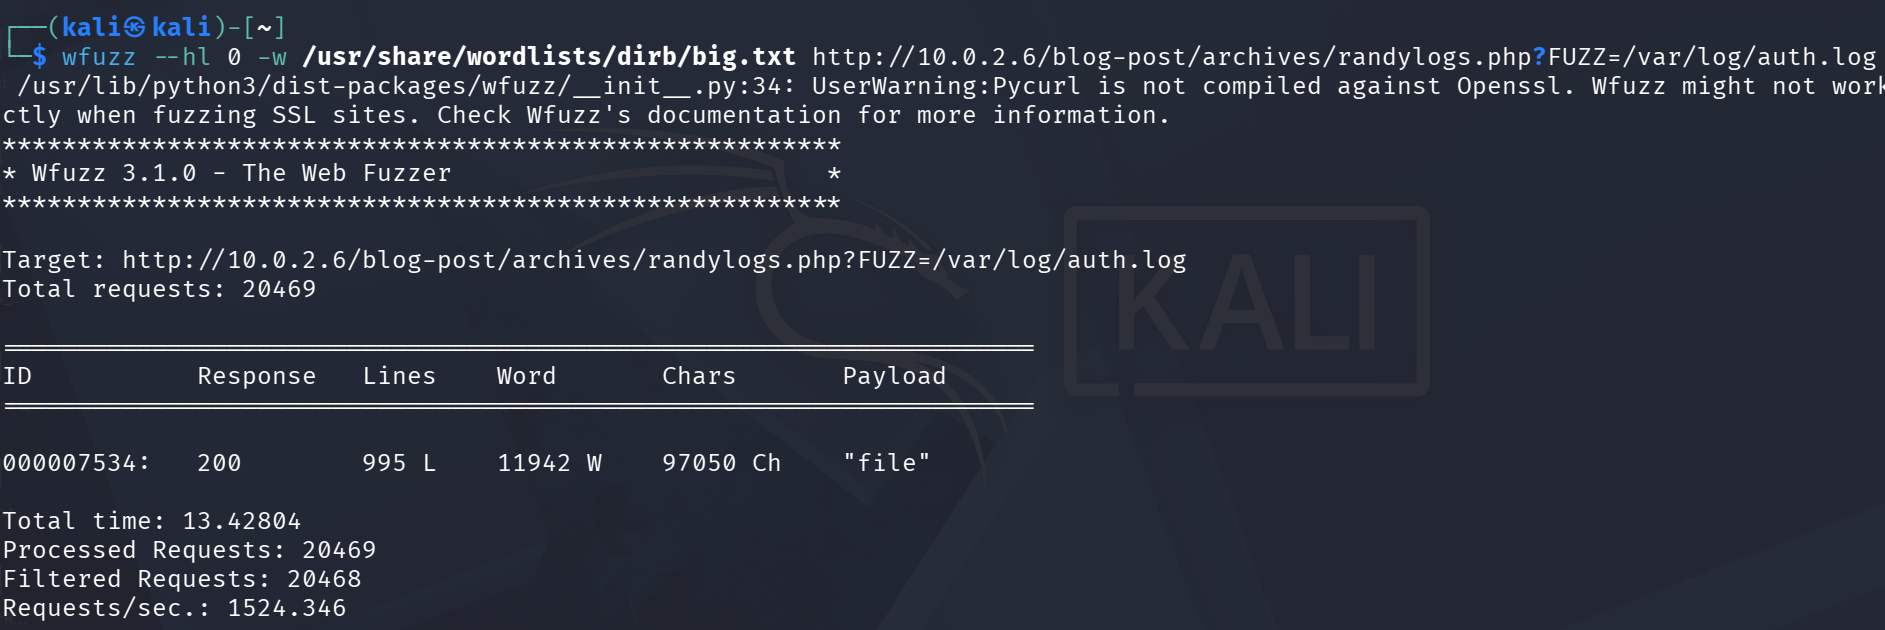
\includegraphics[width=0.75\linewidth]{GlobalAssets/randylogsphpfuzz.png}
\caption{Identification of the \texttt{file} parameter through parameter fuzzing}
\label{fig:detailed-lfi-fuzzing}
\end{figure}

The parameter was subsequently tested using the path to the authentication log referenced by \texttt{tasks\_todo.txt}. The following request successfully retrieved the contents of the local file:

\begin{verbatim}
http://10.0.2.6/blog-post/archives/randylogs.php?file=/var/log/auth.log
\end{verbatim}

\begin{figure}[H]
\centering
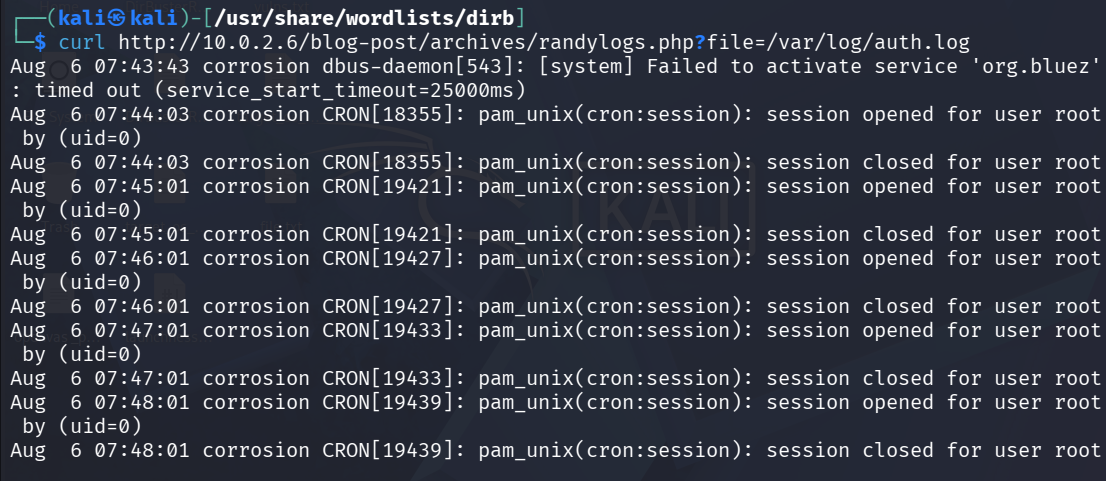
\includegraphics[width=0.75\linewidth]{GlobalAssets/authlogcontent.png}
\caption{Successful retrieval of \texttt{/var/log/auth.log} through the web application}
\label{fig:detailed-authlog}
\end{figure}

This behavior confirms a \textbf{Local File Inclusion (LFI)} vulnerability. The application passes a user-controlled filesystem path to functionality that reads or includes the specified file without enforcing an appropriate restriction on the accessible path.
\\

The impact of this vulnerability is significant because the affected functionality is not restricted to application resources. An attacker can request arbitrary files readable by the web server process, potentially exposing configuration files, credentials, logs, source code, and other sensitive information stored on the underlying operating system.

\subsection{LFI-to-RCE Escalation Through Log Poisoning}

The contents of \texttt{/var/log/auth.log} showed that the file records SSH authentication activity. This introduced the possibility of using the log file as a controllable input source.
\\

The attack consisted of two stages. First, attacker-controlled data had to be written into \texttt{/var/log/auth.log}. Second, the poisoned log had to be processed as PHP code through the existing LFI vulnerability.
\\

An initial attempt was made to inject PHP code through the SSH username field. This approach was unsuccessful because the SSH implementation rejected the characters required to construct the PHP payload.

\begin{figure}[H]
\centering
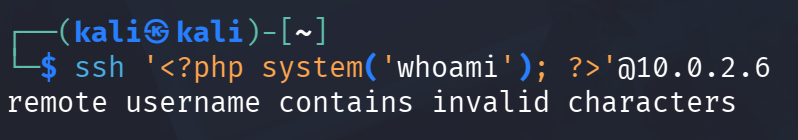
\includegraphics[width=0.75\linewidth]{GlobalAssets/sshinvalidchar.png}
\caption{Unsuccessful attempt to inject PHP code through the SSH username field}
\label{fig:detailed-ssh-injection}
\end{figure}

An alternative method was therefore used to introduce attacker-controlled content into the target environment through the available SFTP functionality. This allowed the required payload to be written to a location subsequently processed through the LFI vulnerability.

\begin{figure}[H]
\centering
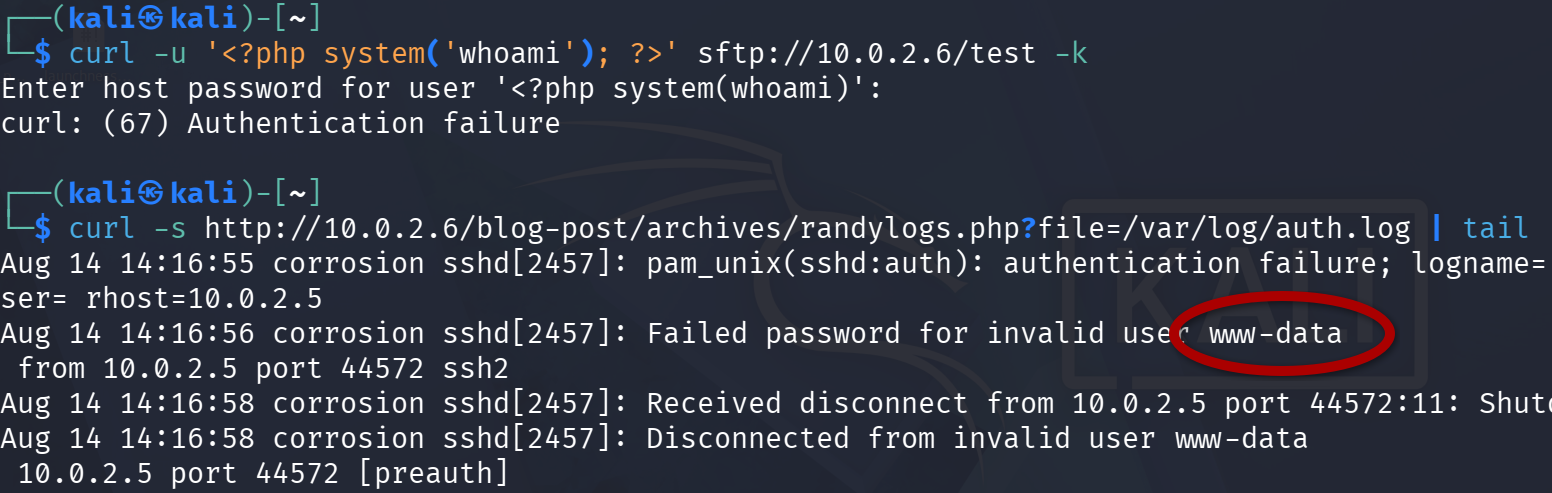
\includegraphics[width=0.75\linewidth]{GlobalAssets/rcesuccess.png}
\caption{Successful exploitation of the LFI vulnerability to achieve code execution}
\label{fig:detailed-lfi-rce}
\end{figure}

The resulting behavior demonstrated that the LFI was not limited to arbitrary file disclosure. Because the included file could contain attacker-controlled PHP code, the vulnerability could be escalated to \textbf{Remote Code Execution (RCE)}.
\\

For exploitation, the injected PHP functionality was designed to accept a second HTTP parameter, \texttt{cmd}, and execute its value using the PHP \texttt{system()} function. This transformed the original arbitrary-file-inclusion primitive into a command-execution primitive.
\\

The resulting attack chain can therefore be summarized as:

\begin{enumerate}
    \item Attacker-controlled input through SFTP;
    \item Poisoned \texttt{/var/log/auth.log} file;
    \item \texttt{randylogs.php?file=<controlled file>};
    \item PHP interpretation of injected content;
    \item Remote command execution.
\end{enumerate}

\subsection{Establishing a Reverse Shell}
To obtain an interactive foothold on the target, a Bash reverse-shell payload was supplied through the \texttt{cmd} parameter. The target was instructed to initiate a TCP connection to the attacking machine at \texttt{10.0.2.5:9000}.
\\

The attacking machine was first configured to listen for the incoming connection using \texttt{netcat}:

\begin{verbatim}
nc -nlvp 9000
\end{verbatim}

\begin{figure}[H]
\centering
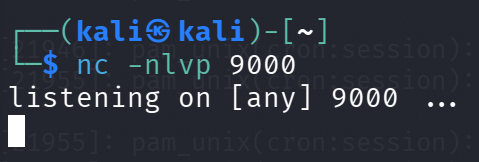
\includegraphics[width=0.50\linewidth]{GlobalAssets/netcat1.png}
\caption{Netcat listener waiting for the reverse-shell connection}
\label{fig:detailed-netcat}
\end{figure}

The malicious command was then supplied to the vulnerable PHP script. When the poisoned file was processed, the injected PHP code executed the command and caused the target to establish the outbound connection.

\begin{figure}[H]
\centering

\includegraphics[width=0.75\linewidth]{GlobalAssets/attackfirefox.png}
\caption{Delivery of the command-execution request}
\label{fig:detailed-request}
\end{figure}

The resulting connection provided an interactive shell on the target system.

\begin{figure}[H]
\centering
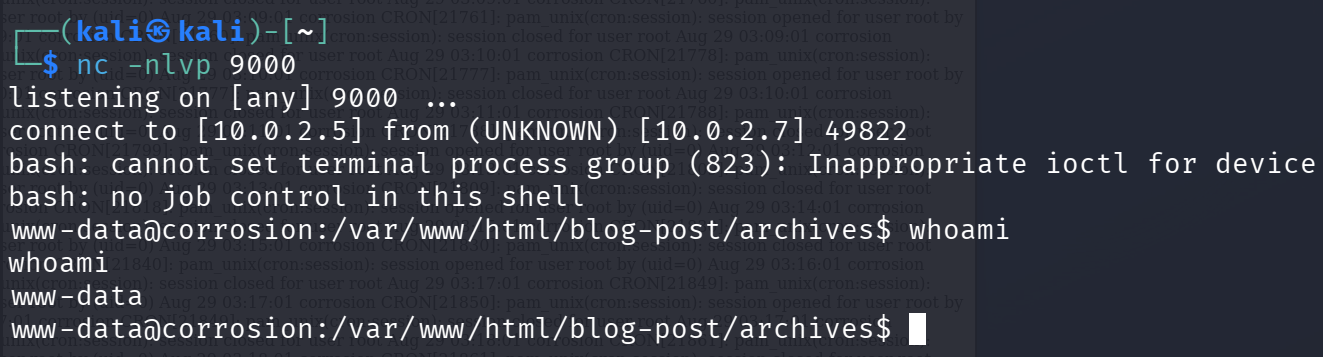
\includegraphics[width=0.75\linewidth]{GlobalAssets/reverseshellsuccess.png}
\caption{Successful establishment of the reverse shell}
\label{fig:detailed-reverse-shell}
\end{figure}

At this stage, remote code execution had been successfully converted into an interactive foothold on the target. The shell initially operated with the privileges of the web application process, providing a low-privileged context from which local privilege escalation and further enumeration could be performed.

\subsection{Post-Exploitation and Credential Discovery}

Following establishment of the reverse shell, local enumeration was performed to identify users, sensitive files, and potential privilege escalation vectors.
\\

Inspection of \texttt{/etc/passwd} revealed the presence of the \texttt{randy} user account.

\begin{figure}[H]
\centering
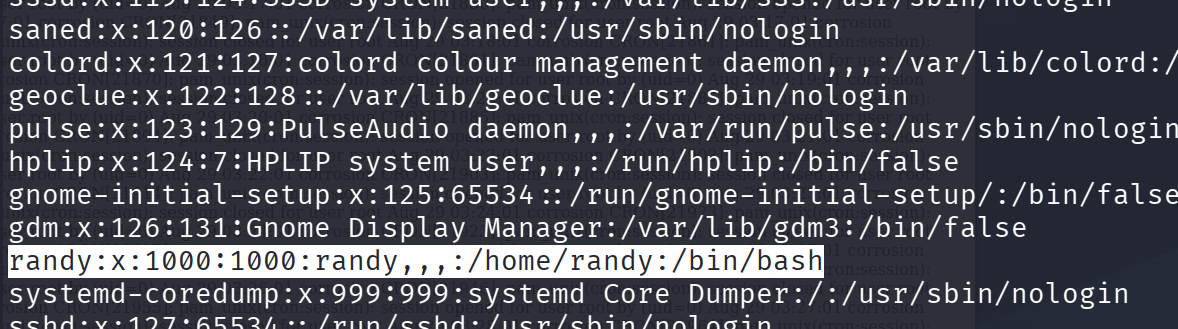
\includegraphics[width=0.75\linewidth]{GlobalAssets/userrandy.png}
\caption{Identification of the \texttt{randy} user account}
\label{fig:detailed-randy}
\end{figure}

Further filesystem enumeration identified \texttt{user\_backup.zip} within \texttt{/var/backups/}. The archive was password-protected and could not initially be extracted.

\begin{figure}[H]
\centering
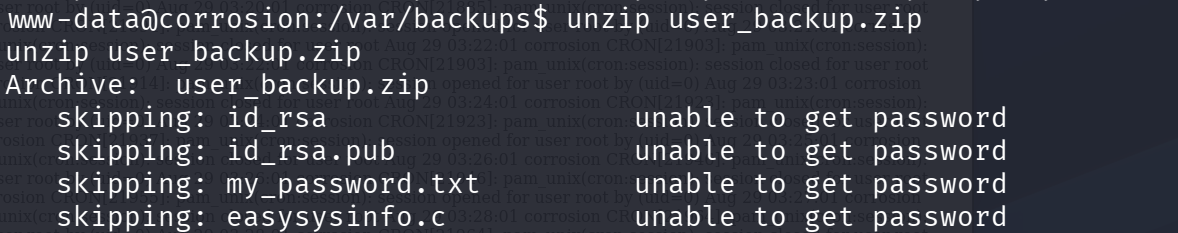
\includegraphics[width=0.75\linewidth]{GlobalAssets/unzipfail.png}
\caption{Password protection preventing extraction of \texttt{user\_backup.zip}}
\label{fig:detailed-zip-protected}
\end{figure}

Because the archive was accessible from the compromised system and potentially contained authentication material, it was selected for further analysis.
\\

The archive was transferred to the attacking machine and subjected to password recovery using \texttt{zip2john} and \texttt{John the Ripper}. The password was successfully recovered.

\begin{figure}[H]
\centering
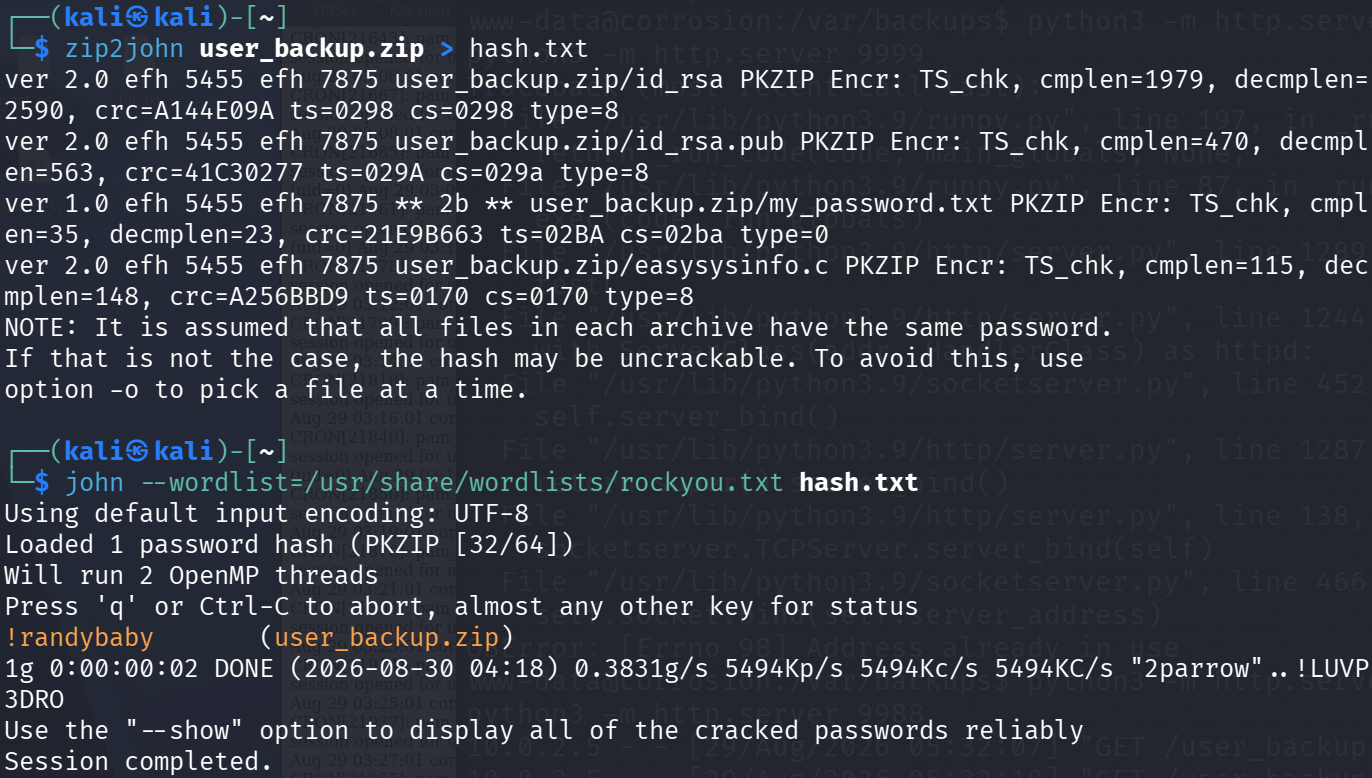
\includegraphics[width=0.75\linewidth]{GlobalAssets/randybaby.png}
\caption{Recovery of the password protecting the backup archive}
\label{fig:detailed-password-cracking}
\end{figure}

Extraction of the archive revealed several sensitive files:

\begin{itemize}
\item \texttt{id\_rsa}, containing a private SSH key;
\item \texttt{id\_rsa.pub}, containing the corresponding public key;
\item \texttt{my\_password.txt}, containing a user password;
\item \texttt{easysysinfo.c}, containing the source code of a privileged utility.
\end{itemize}

\begin{figure}[H]
\centering
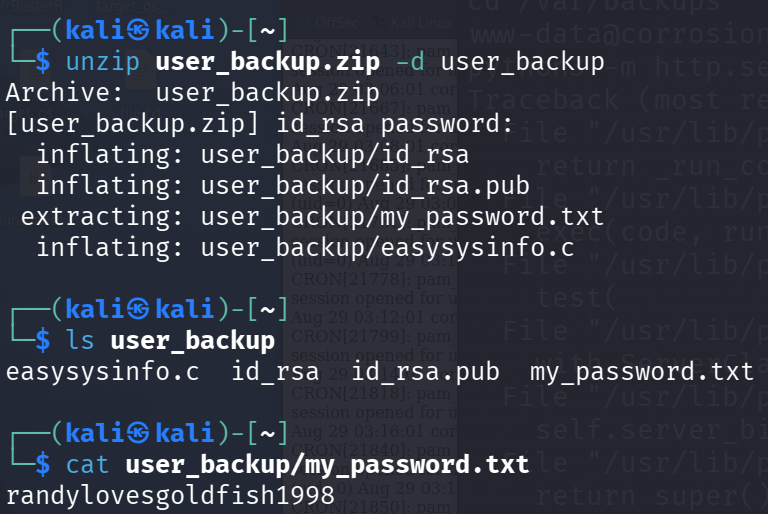
\includegraphics[width=0.50\linewidth]{GlobalAssets/zipcracked.png}
\caption{Sensitive contents recovered from \texttt{user\_backup.zip}}
\label{fig:detailed-zip-content}
\end{figure}

The password contained in \texttt{my\_password.txt} enabled authentication to the \texttt{randy} account.

\begin{figure}[H]
\centering
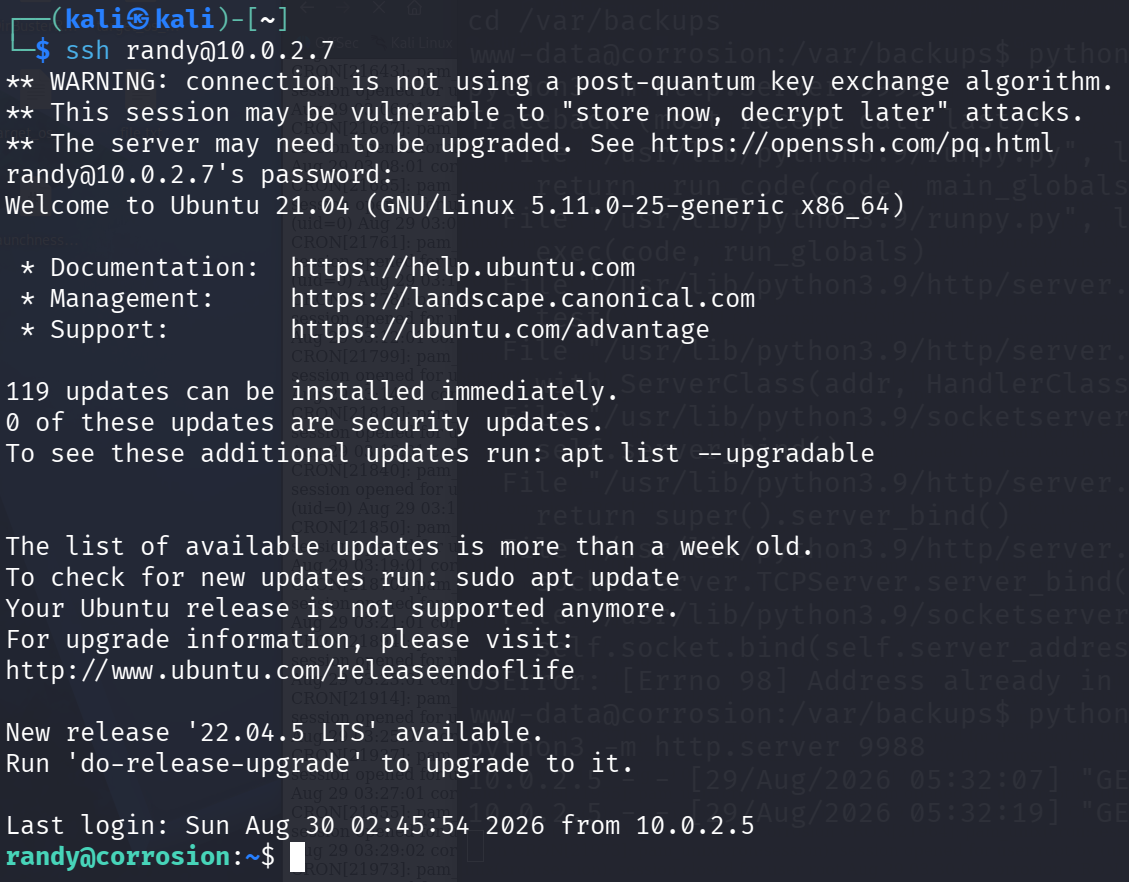
\includegraphics[width=0.75\linewidth]{GlobalAssets/randylogin.png}
\caption{Successful authentication as the \texttt{randy} user}
\label{fig:detailed-randy-login}
\end{figure}

This represented a privilege transition from the web application's low-privileged execution context to a legitimate local user account.

\subsection{Local Privilege Escalation}

Enumeration of the \texttt{randy} user's environment identified the \texttt{easysysinfo} utility within the user's \texttt{tools} directory.

\begin{figure}[H]
\centering
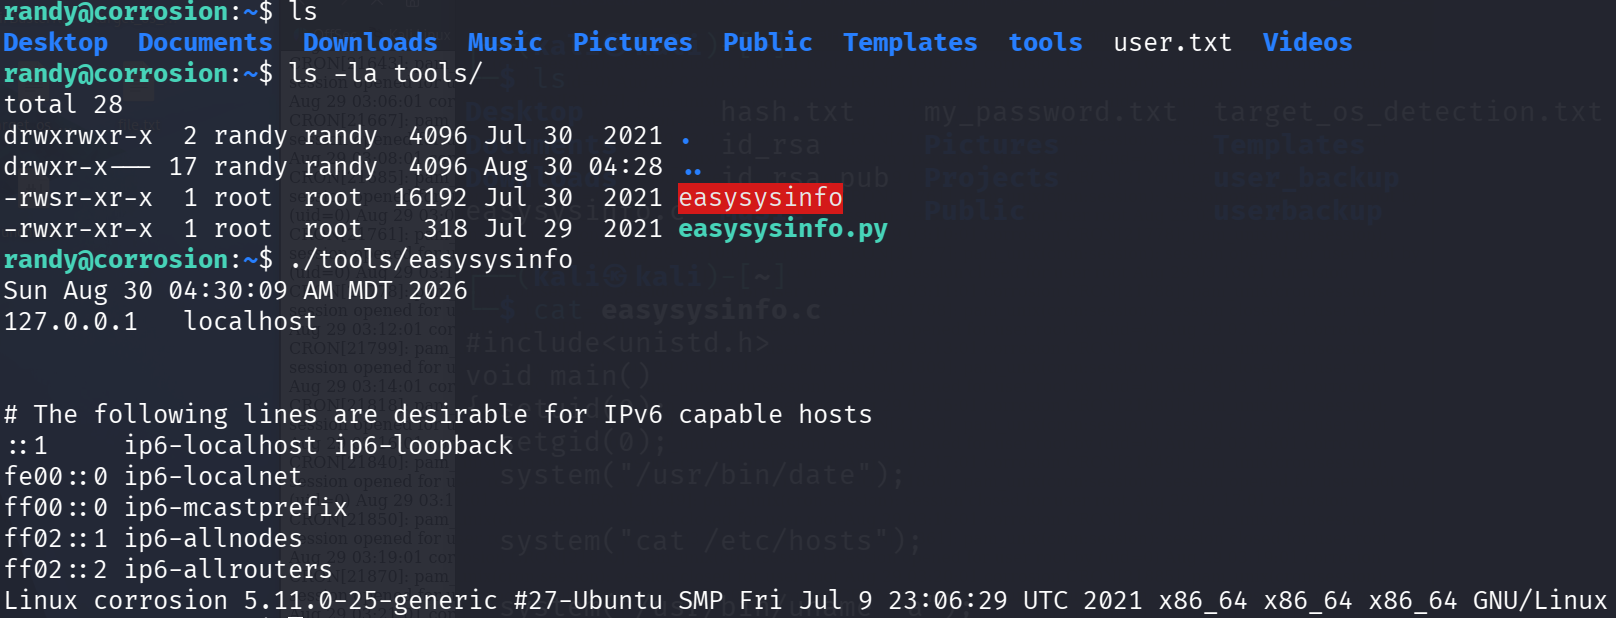
\includegraphics[width=0.75\linewidth]{GlobalAssets/exploring.png}
\caption{Enumeration of the \texttt{randy} user's environment}
\label{fig:detailed-randy-enumeration}
\end{figure}

The executable had \texttt{setuid} permissions, meaning that it executed with the effective privileges of its file owner rather than solely with the privileges of the invoking user. 
\\

Further analysis showed that the program was owned by \texttt{root} and therefore represented a potential privilege escalation vector.
\\

The corresponding source code found in the \texttt{user\_backup.zip} archive revealed the use of the C \texttt{system()} function to invoke the \texttt{cat} utility.

\begin{figure}[H]
\centering
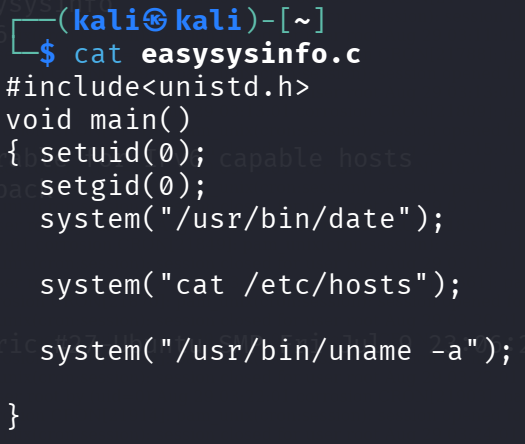
\includegraphics[width=0.40\linewidth]{GlobalAssets/easysysinfo.png}
\caption{Source code of the \texttt{easysysinfo} utility}
\label{fig:detailed-easysysinfo}
\end{figure}

The security weakness results from the use of an external executable without specifying its absolute filesystem path. Instead of explicitly invoking a trusted executable such as \texttt{/bin/cat}, the program relies on the \texttt{PATH} environment variable to determine which executable should be executed.
\\

This behavior is classified as \textbf{CWE-426: Untrusted Search Path}. An attacker able to influence the execution environment can cause a malicious executable to be resolved in place of the intended system binary.
\\

Because the vulnerable program executes with root privileges, successful manipulation of executable resolution causes the attacker-controlled program to inherit those privileges.

\subsection{Root Privilege Escalation}

To demonstrate the impact of the vulnerable search-path behavior, a malicious executable named \texttt{cat} was created.

\begin{figure}[H]
\centering
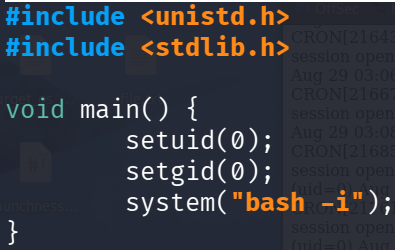
\includegraphics[width=0.40\linewidth]{GlobalAssets/fakecat.png}
\caption{Creation of the malicious \texttt{cat} executable}
\label{fig:detailed-fakecat}
\end{figure}

The executable was placed in \texttt{/tmp}, and the \texttt{PATH} environment variable was modified so that \texttt{/tmp} was searched before the directory containing the legitimate \texttt{cat} executable.
\\

Consequently, when \texttt{easysysinfo} invoked \texttt{cat}, the malicious executable was resolved instead of the legitimate system binary.
\\

Since \texttt{easysysinfo} executes with root privileges, the attacker-controlled process inherited the corresponding effective privileges. Execution of the utility therefore resulted in a \textbf{root shell}.

\begin{figure}[H]
\centering
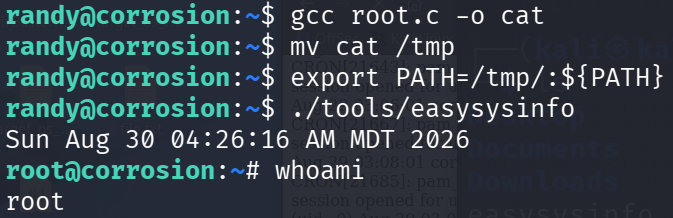
\includegraphics[width=0.75\linewidth]{GlobalAssets/rooted.png}
\caption{Successful local privilege escalation to root}
\label{fig:detailed-root}
\end{figure}

The successful privilege escalation demonstrates that the initial web application compromise could ultimately be converted into complete operating-system-level takeover.




%------------------------------------------------
% Back matter
%------------------------------------------------
\clearpage
\pagenumbering{Alph}

\printbibliography

\end{document}